\section[Factoring Out Symmetries in Concentration Profiles]{Factoring Out Symmetries in Concentration Profiles}

\begin{frame}{Importance of Symmetries in Data Analysis}
	
	\drawunordered
	
	\drawdownarrow
	
	\draworderedvdm
	    
	Note that the images are not only ordered, but also {\bf aligned}.
	
	We must {\em factor out} rotational symmetries before (or in conjunction with) ordering the images. 
	

\end{frame}

%\begin{frame}{Importance of Symmetries in Data Analysis}
%
%	\centering
%	In the previous analysis, we first needed to determine \\where to open and ``unroll'' the circle to obtain a linear profile.
%	
%	\centering
%	\begin{tikzpicture}
%		\node (drosophila_line) {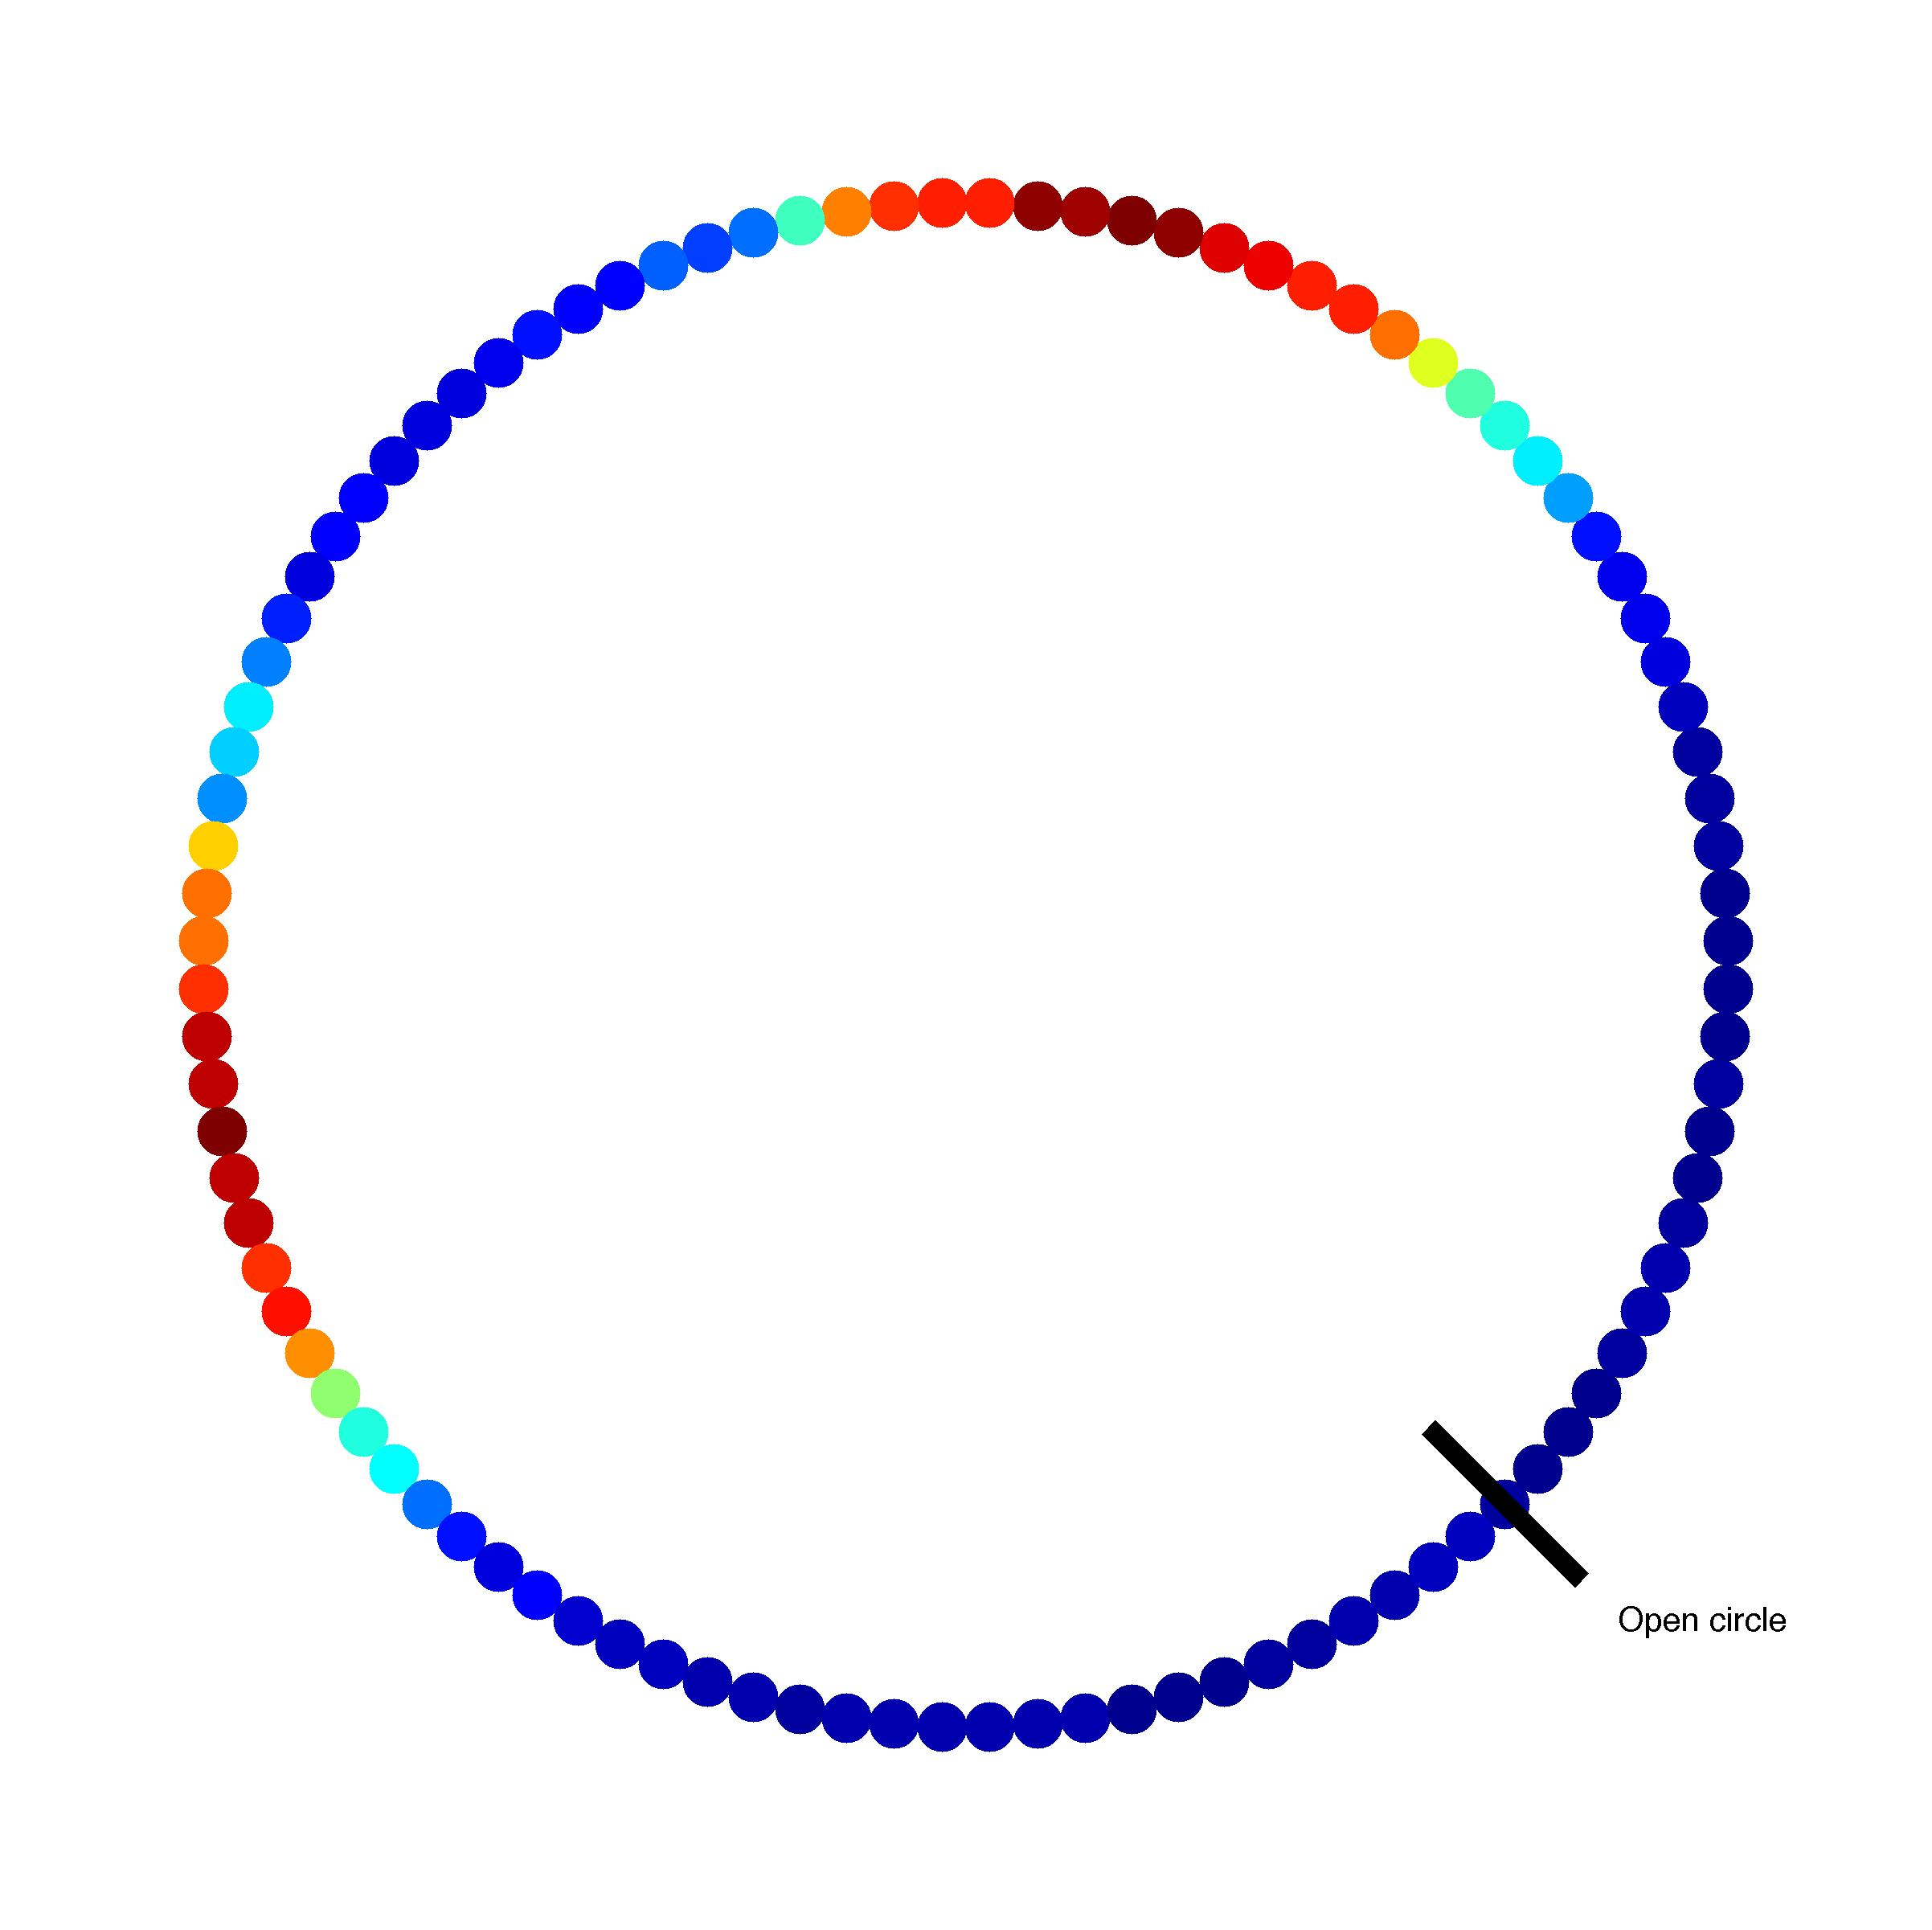
\includegraphics[width=0.2\textwidth]{circle_profile}};
%		\node[right=0.3\textwidth of drosophila_line] (drosophila_circle) {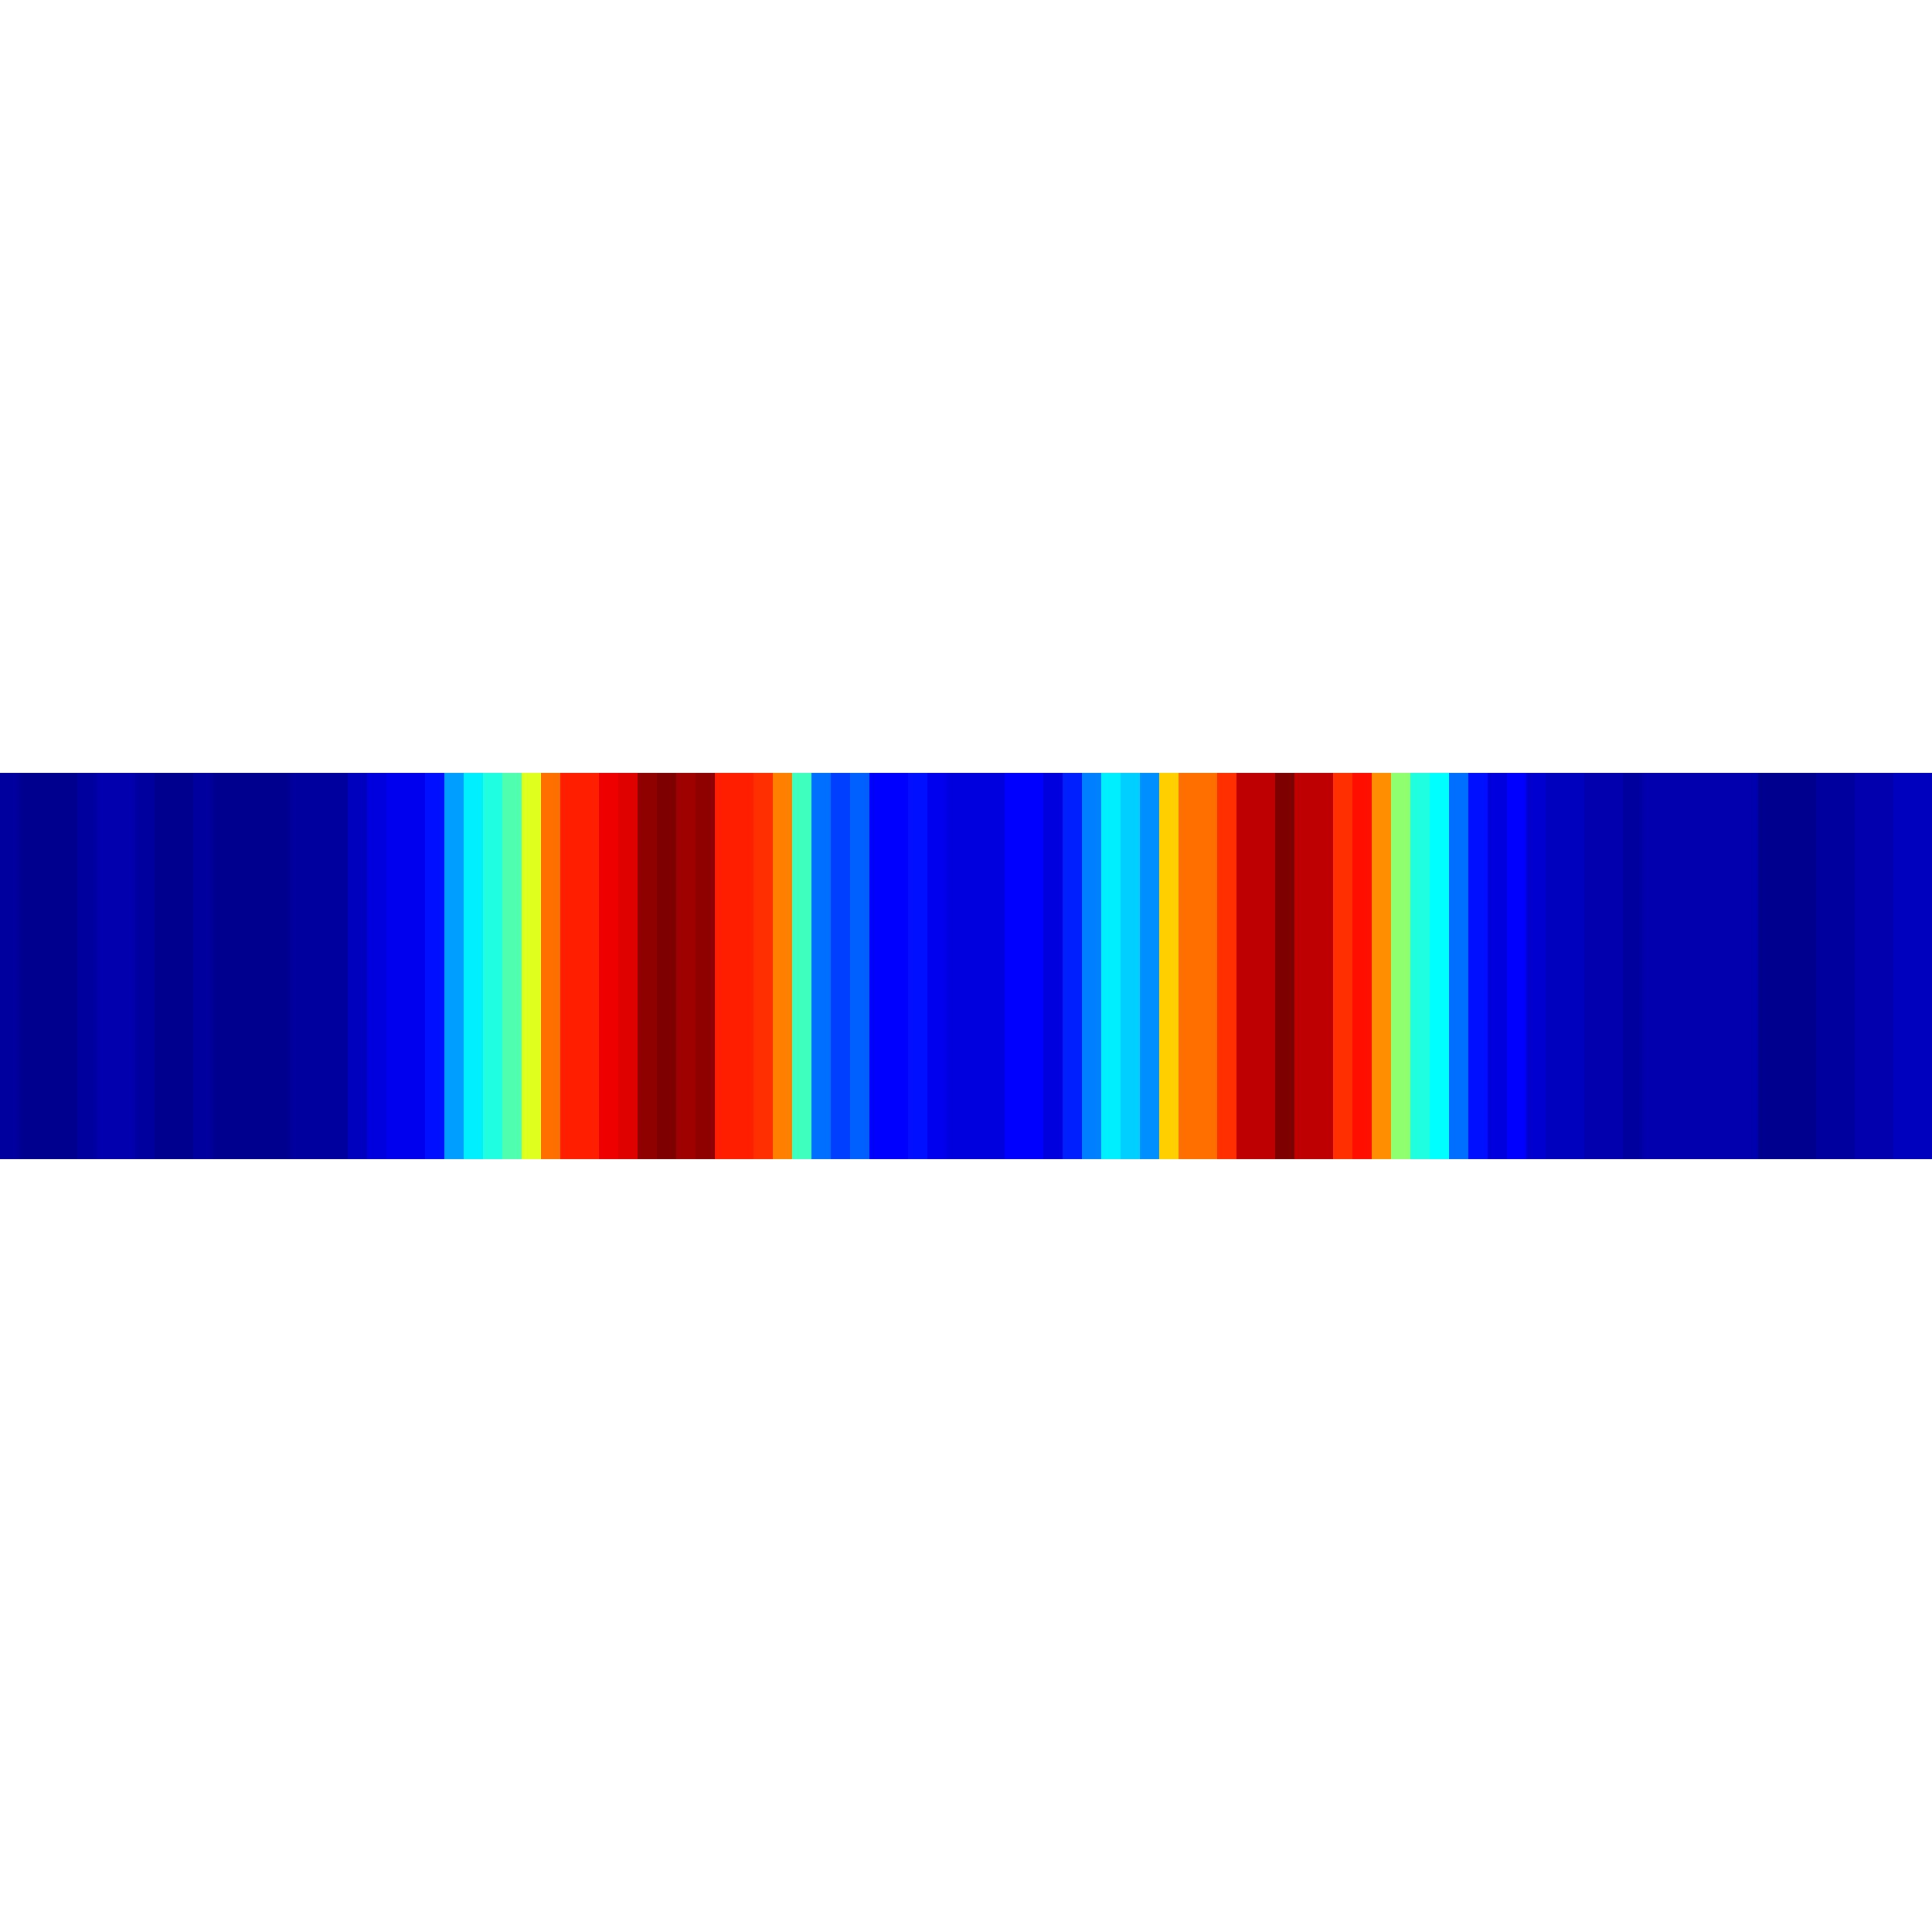
\includegraphics[width=0.25\textwidth, height=0.1in]{line_profile}};
%		\draw[->] (drosophila_line) -- (drosophila_circle) node[above,midway] {``Unroll'' circle};
%	\end{tikzpicture}
%	
%	This is done by staining for {\em another} protein (Dorsal) that is expressed only along the ventral midline, and opening each profile at its dorsal midline. 
%	
%	\vspace{0.2in}
%	
%	Instead, we would like to work {\em directly} with the circular concentration profiles, \\ and align the concentration profiles {\em automatically}, \\without staining for a second protein. 
%
%\end{frame}

\begin{frame}[t]{Aligning Images Under Rotations}
	
	\begin{itemize}
	\item We assume that we have many {\em rotated} copies of {\em the same} image.
	%
	\item We would like to align the images so that we can perform further analysis that will be {\em invariant} to rotations. 
	%
	\item This is essential for our {\em Drosophila} data, because the developmental dynamics are invariant to the orientation of the embryos in the microfluidic device.
	\end{itemize}

	\centering
	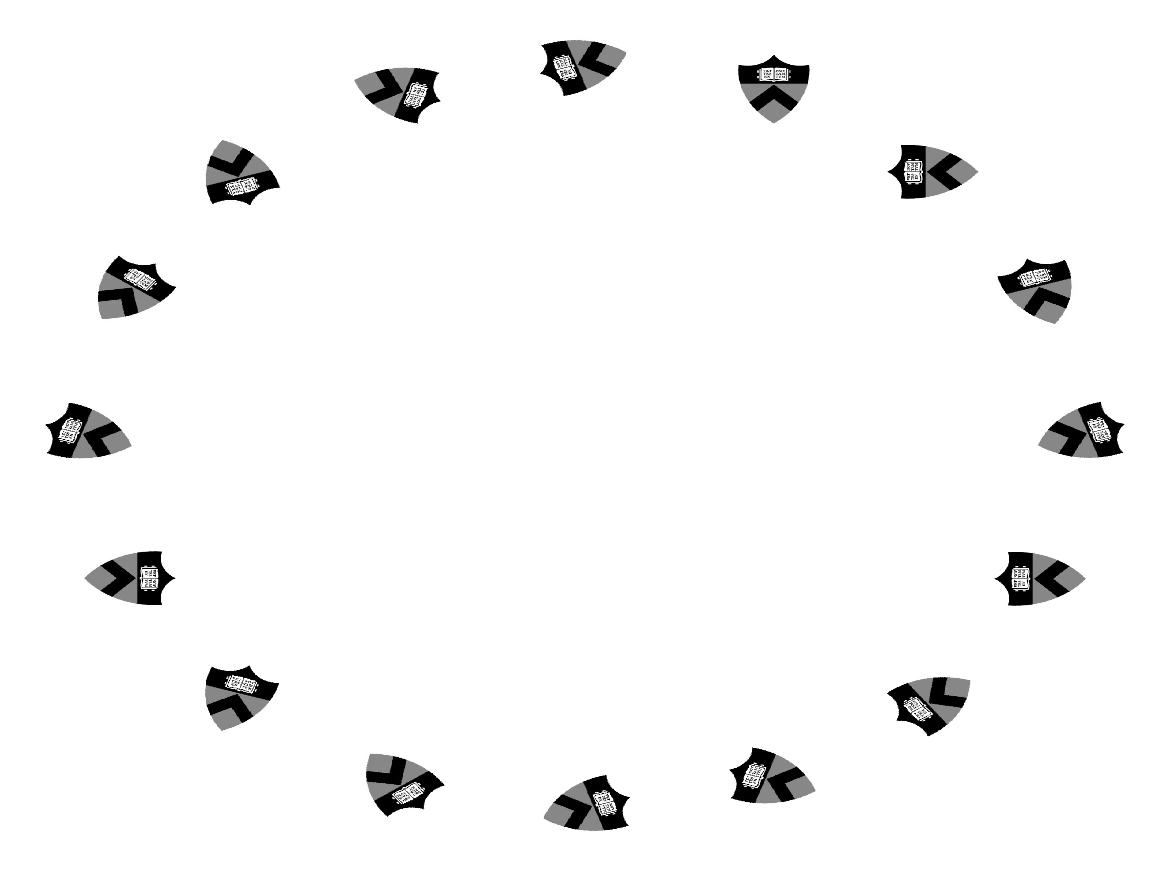
\includegraphics[width=0.5\textwidth]{PU_clean}\\
	{\scriptsize Many rotated copies of the Princeton University shield. \\ We will use this to illustrate different alignment algorithms. \par}	

\end{frame}

\begin{frame}[t]{Template-Based Alignment}
	\centering	
	
	If we have many images and wish to align them, \\ we can rotate each one until it is optimally aligned with a {\bf template}.

	In this case, we have chosen the template to be one of the images in the dataset.

	\only<1>{
		\begin{tikzpicture}
		\node (fig1) {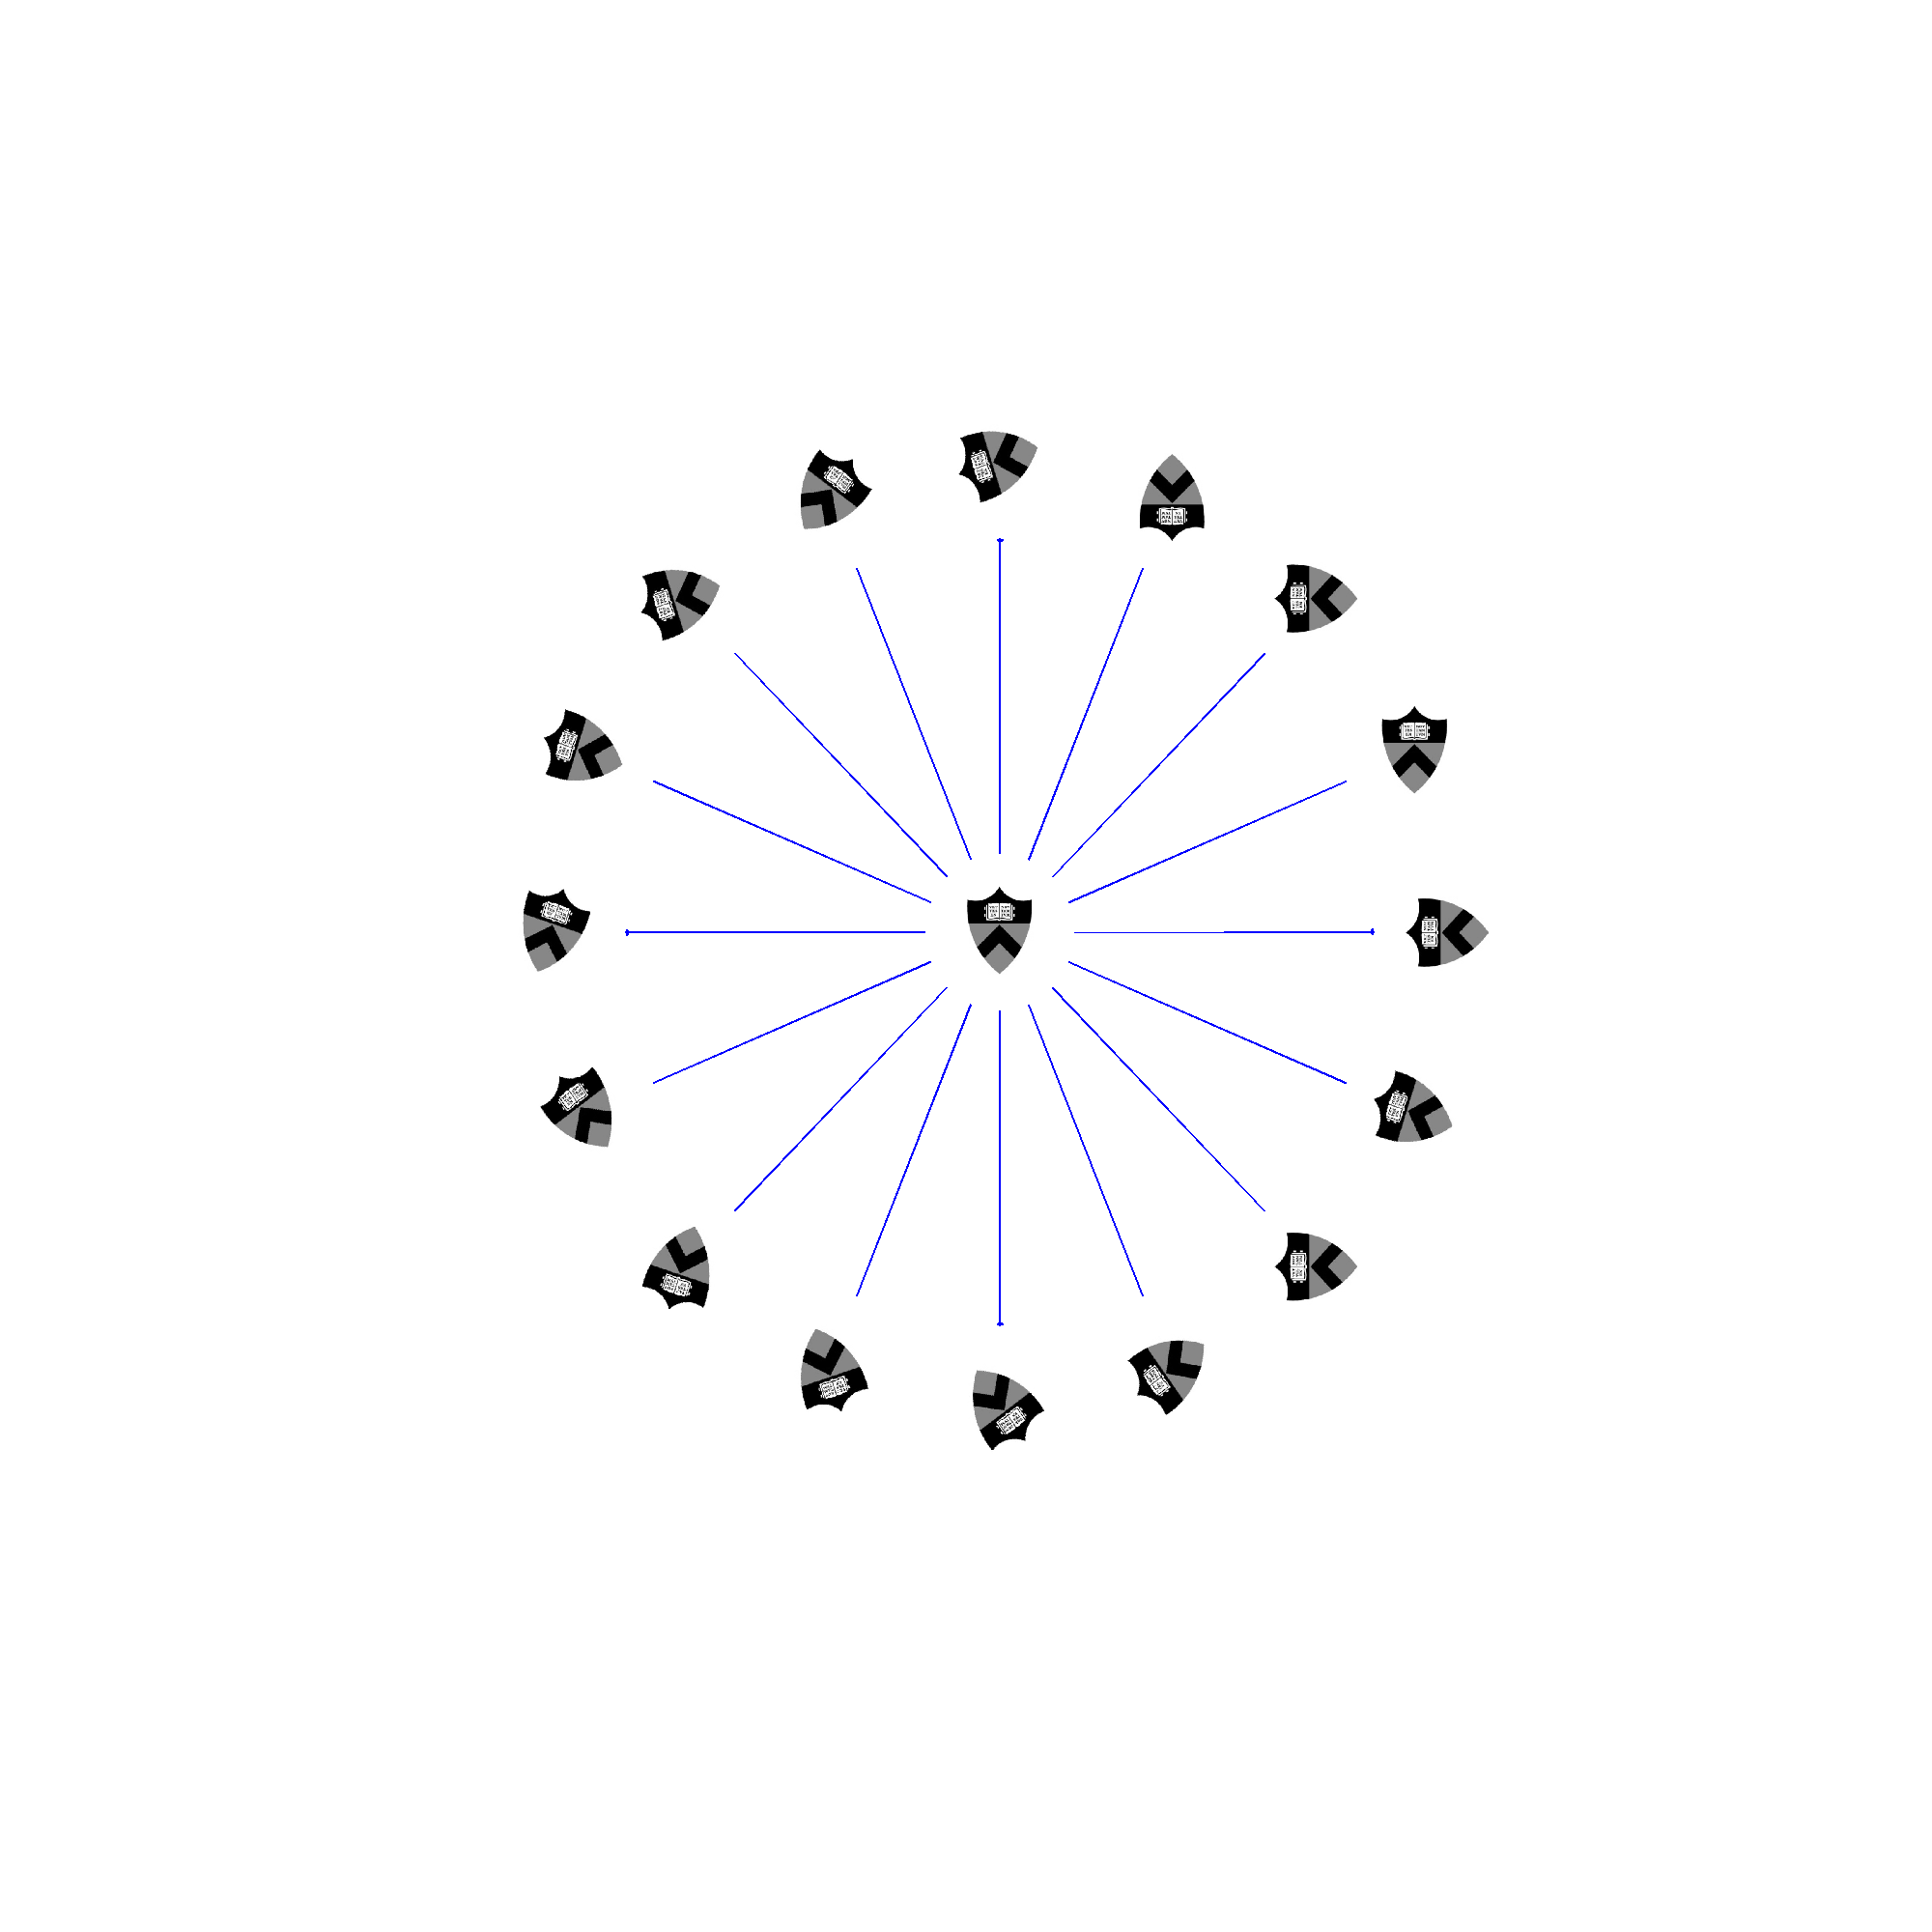
\includegraphics[width=0.6\textwidth]{PU_template1_clean}};
		\draw [red] (-0.31,-0.31) rectangle (0.31,0.31);
		\draw [red] (0.89, 1.89) rectangle (1.49,2.49);		
		\end{tikzpicture}
		\\
	{\small \em Images, unaligned. The template is shown in the center. \par}}
	\only<2>{
		\begin{tikzpicture}
		\node (fig1) {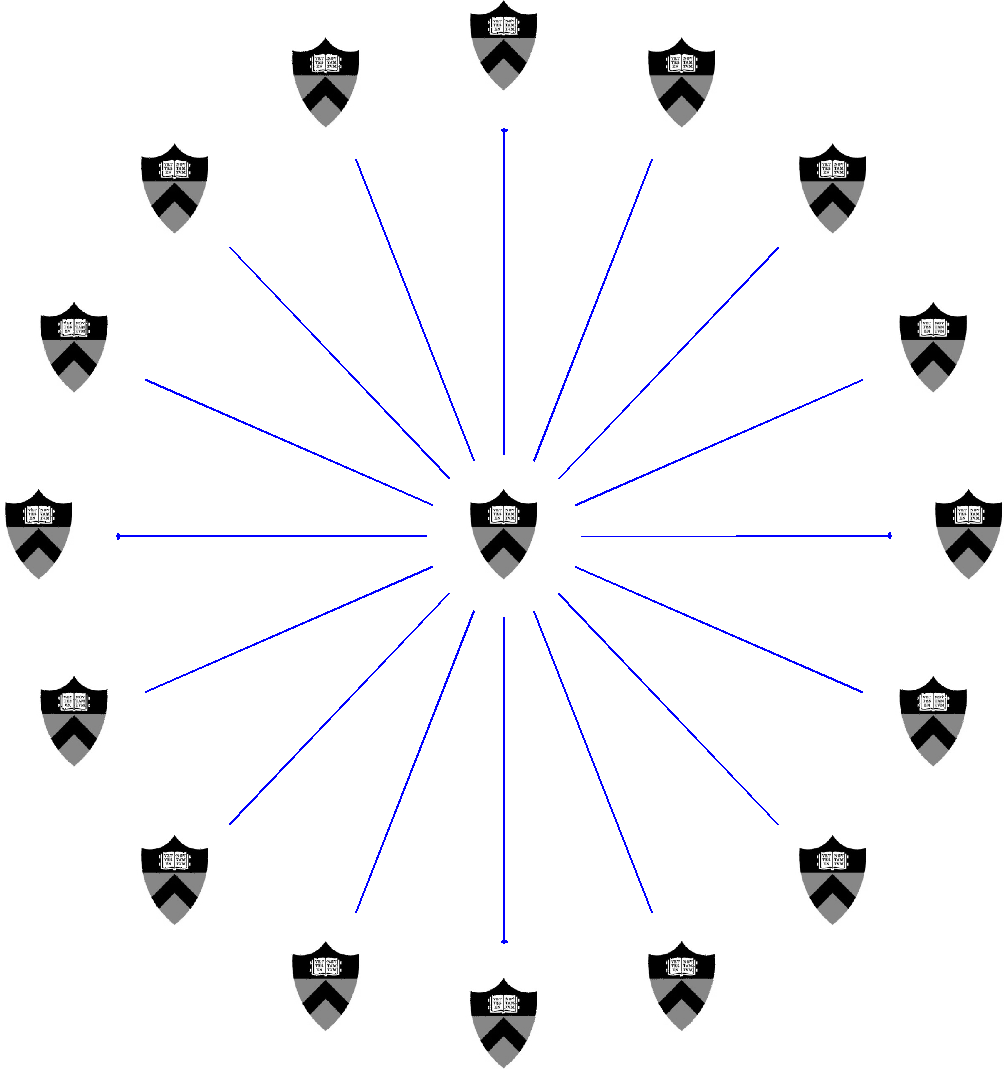
\includegraphics[width=0.6\textwidth]{PU_template2_clean}};
		%\draw [red] (-0.31,-0.31) rectangle (0.31,0.31);
		%\draw [red] (0.89, 1.89) rectangle (1.49,2.49);		
		\end{tikzpicture}
		\\
	{\small \em Images, aligned to template. The template is shown in the center. \par}}
		
\end{frame}

\begin{frame}[t]{Template-Based Alignment Under Noisy Conditions}

	\centering
	However, if the images are noisy, 
	\\then template-based alignment will often be inaccurate.

	\only<1>{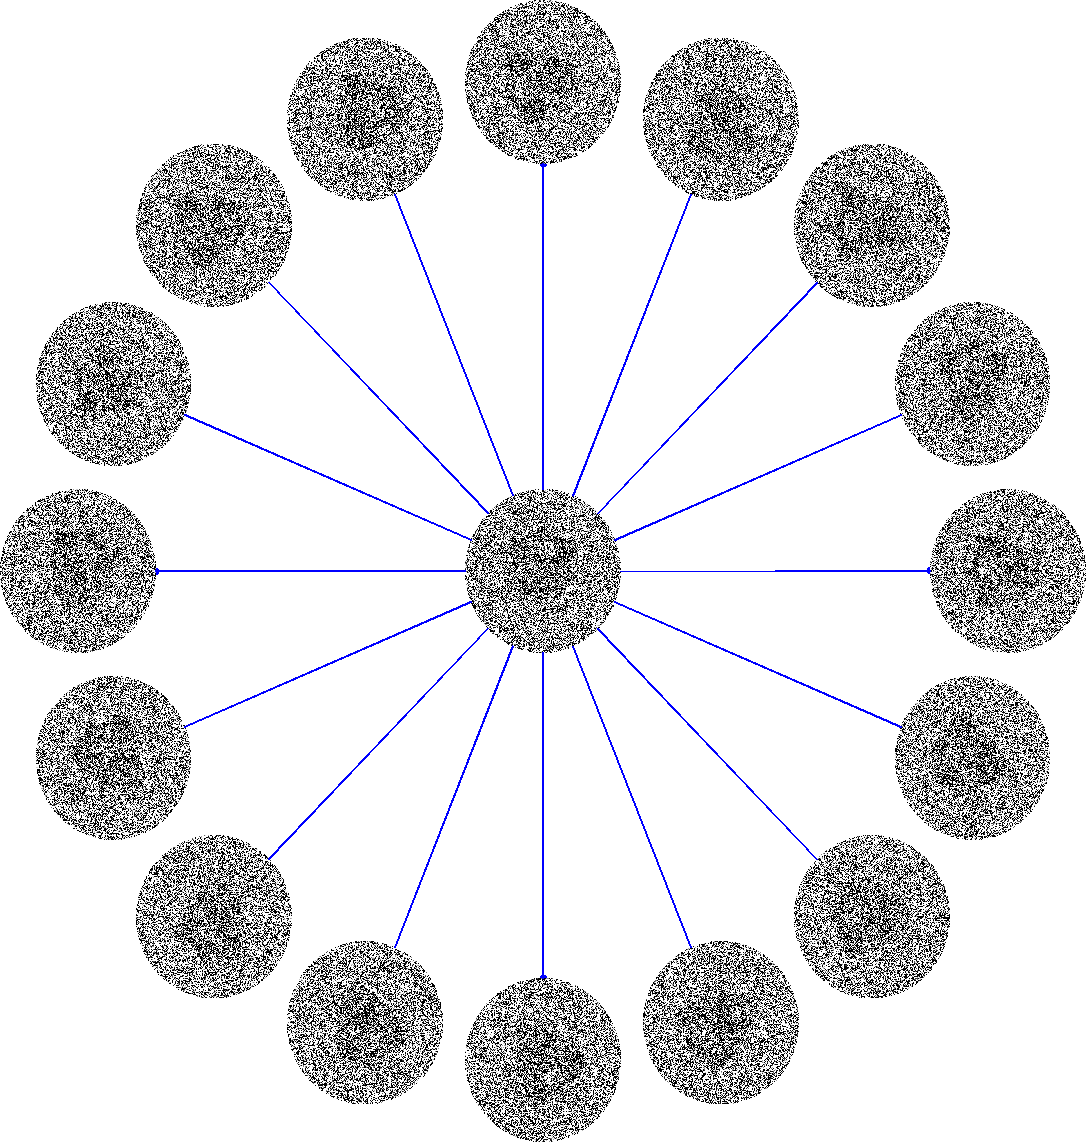
\includegraphics[width=0.6\textwidth]{PU_template1_noisy}\\
	{\small \em Images, unaligned, now corrupted with white Gaussian noise. \\ The template is shown in the center. \par}}
	\only<2>{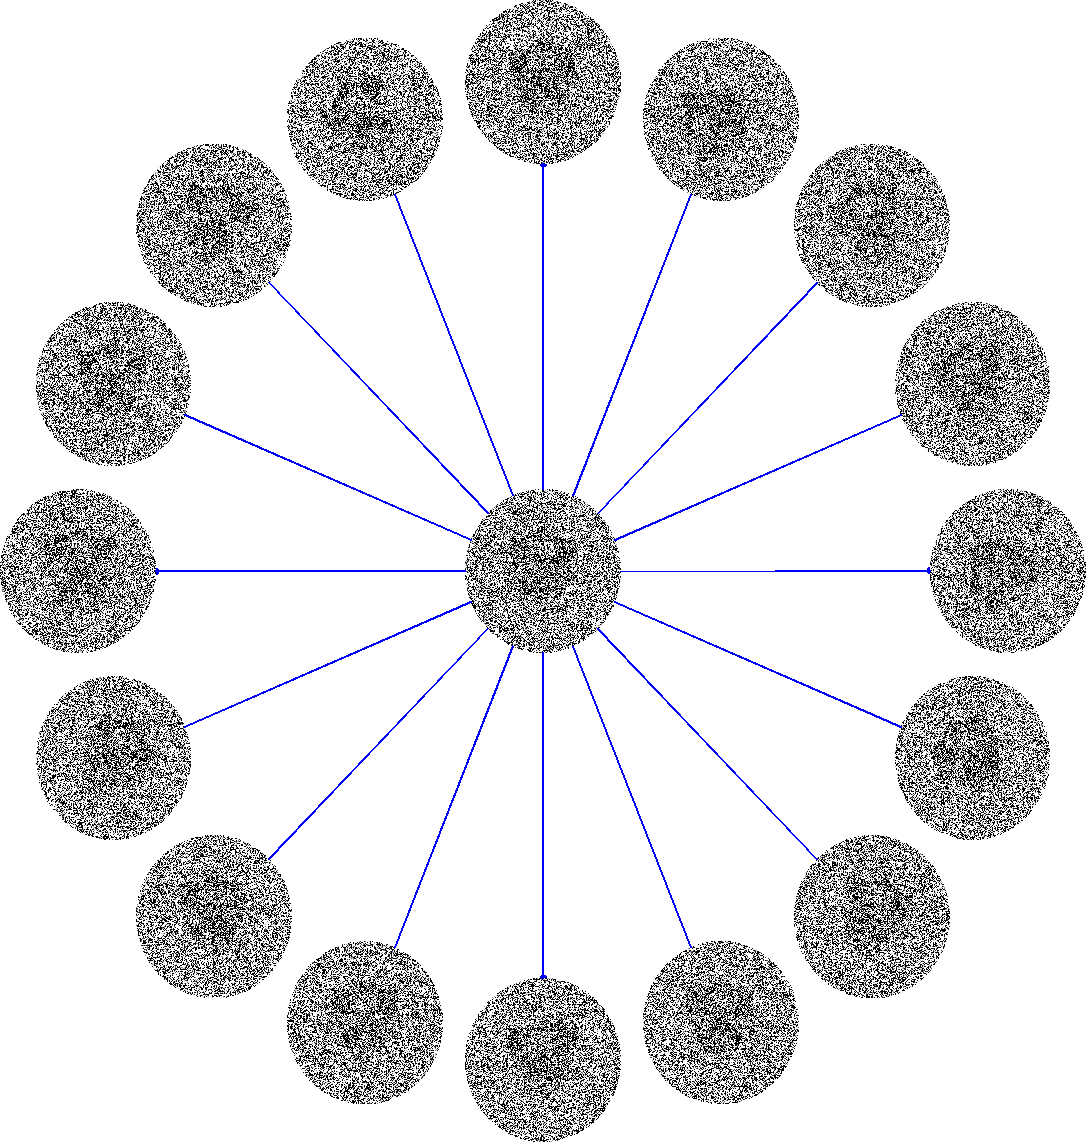
\includegraphics[width=0.6\textwidth]{PU_template2_noisy}\\
	{\small \em Images, aligned to template. The template is shown in the center. \par}}
	\only<3>{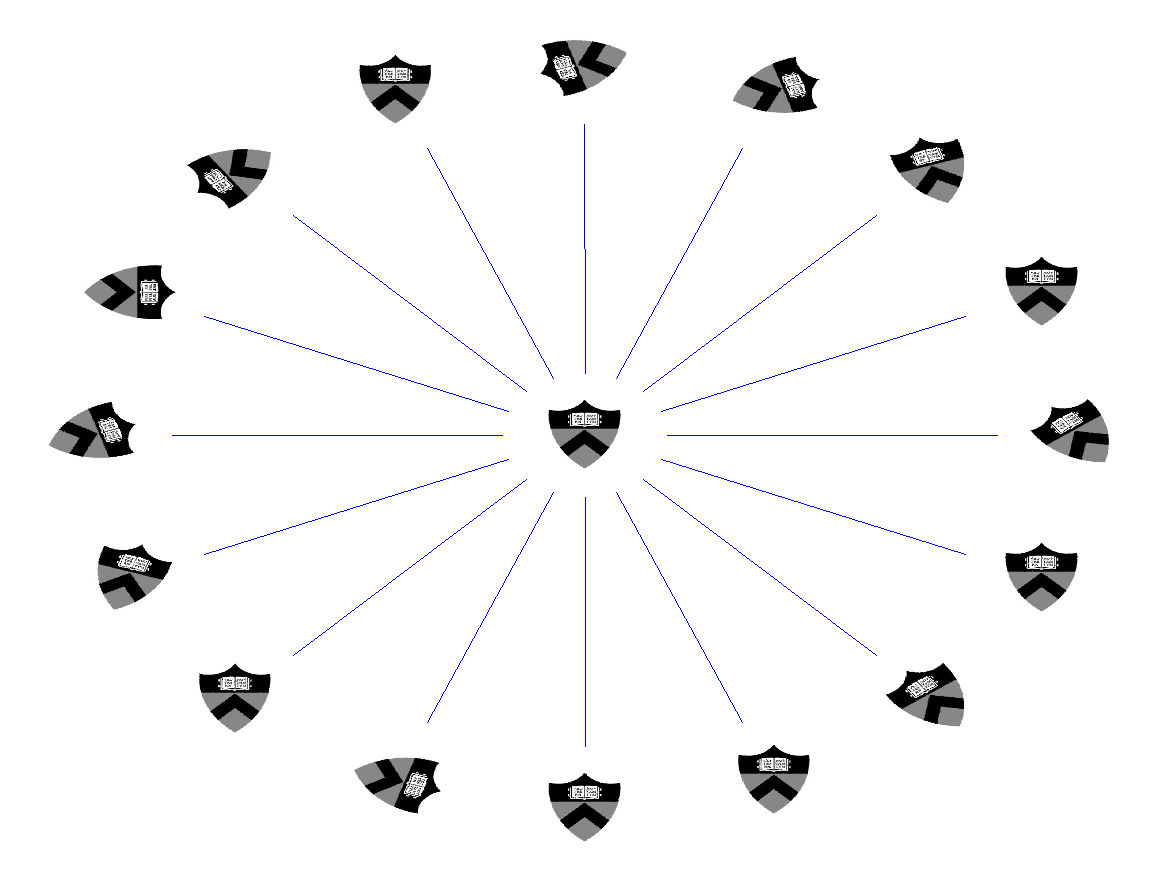
\includegraphics[width=0.6\textwidth]{PU_template3_noisy}\\
	{\small \em Images, denoised after being aligned to template. The template is shown in the center. Note that there are several misalignments. \par}}
	
\end{frame}

\begin{frame}[t]{Issues with Template Alignment: Consistency}

	\centering
	The rotations that we compute should be {\em consistent} with each other. 
		
	\vspace{0.1in}
	
	%\begin{overpic}[width=0.6\textwidth,grid,tics=10]{PU_consistency_noisy}	
	\begin{overpic}[width=0.6\textwidth]{PU_consistency_noisy}
 	\put (90,15) {\scriptsize $270^{\circ} + 252 ^{\circ} \neq 342^{\circ}$}
	\end{overpic}
	
Inconsistencies indicate that there are errors in our alignments.
	
	We would like to use {\em all} pairwise alignments in calculating the {\em optimal} rotation for each image, and trust those pairwise alignments that are {\em most consistent}.
	
\end{frame}

\begin{frame}[t]{Angular Synchronization for Alignment}
	
	Instead, we would like to use each image as a template for every other image, and~then find the most {\em consistent} set of alignments. \\ This is called {\bf angular synchronization} \footcite{singer2011angular}.
	
	\begin{minipage}[t]{0.55\textwidth}	
	\vspace{0in}
	\centering
	\only<1>{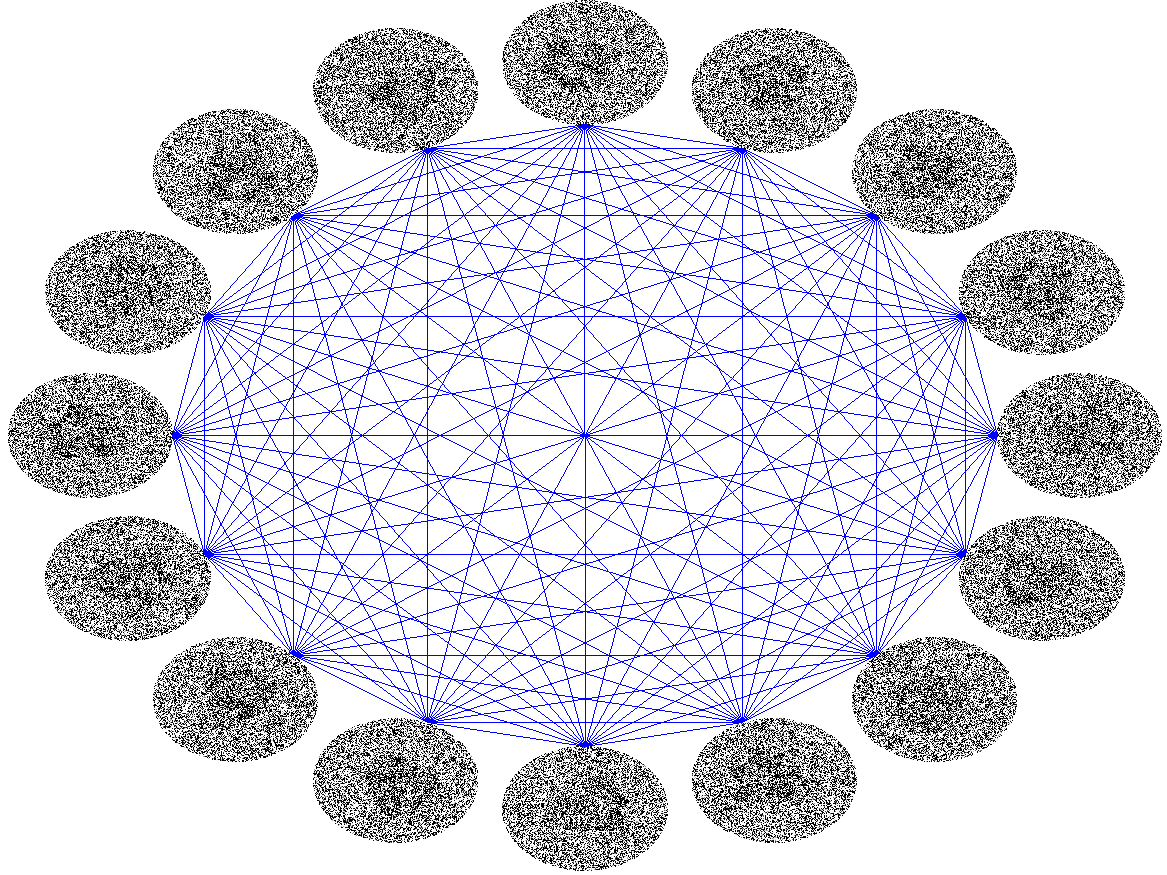
\includegraphics[width=0.9\textwidth]{PU_angsynch1} \\
	{\small \em Images, unaligned, \\now corrupted with white Gaussian noise. \par}}
	\only<2>{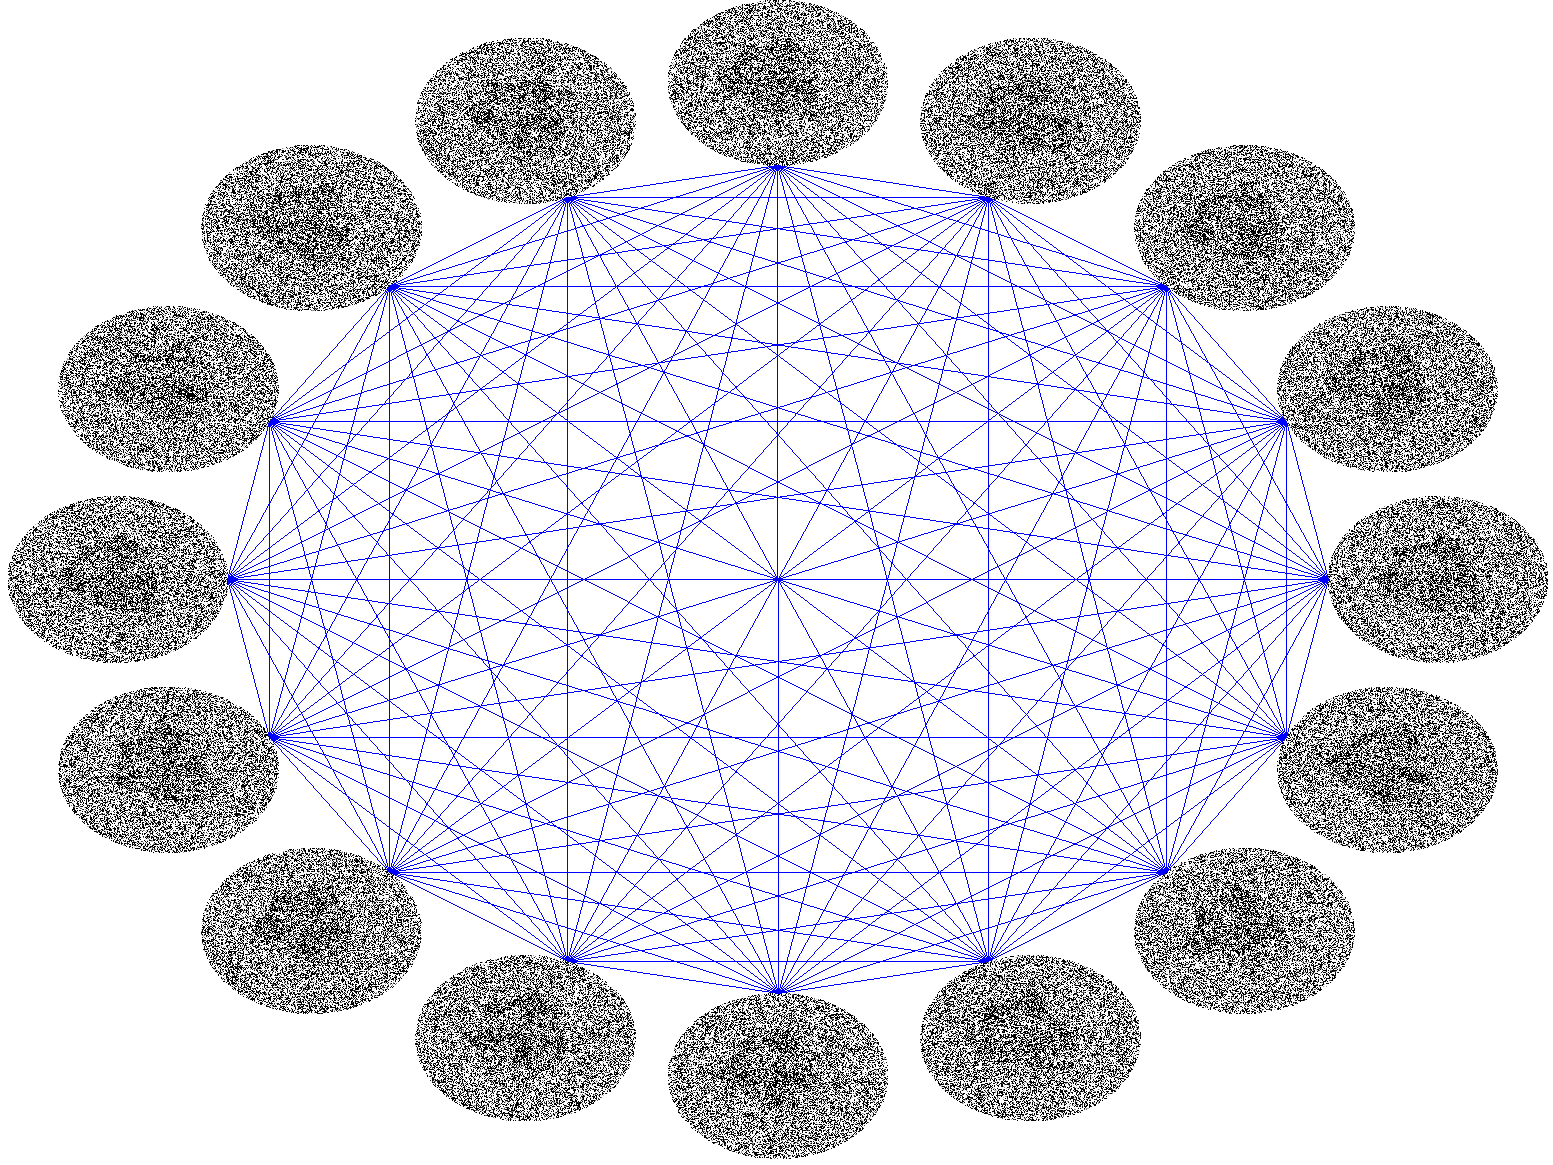
\includegraphics[width=0.9\textwidth]{PU_angsynch2}\\
	{\small \em Images, aligned using angular synchronization. \par}}
	\only<3>{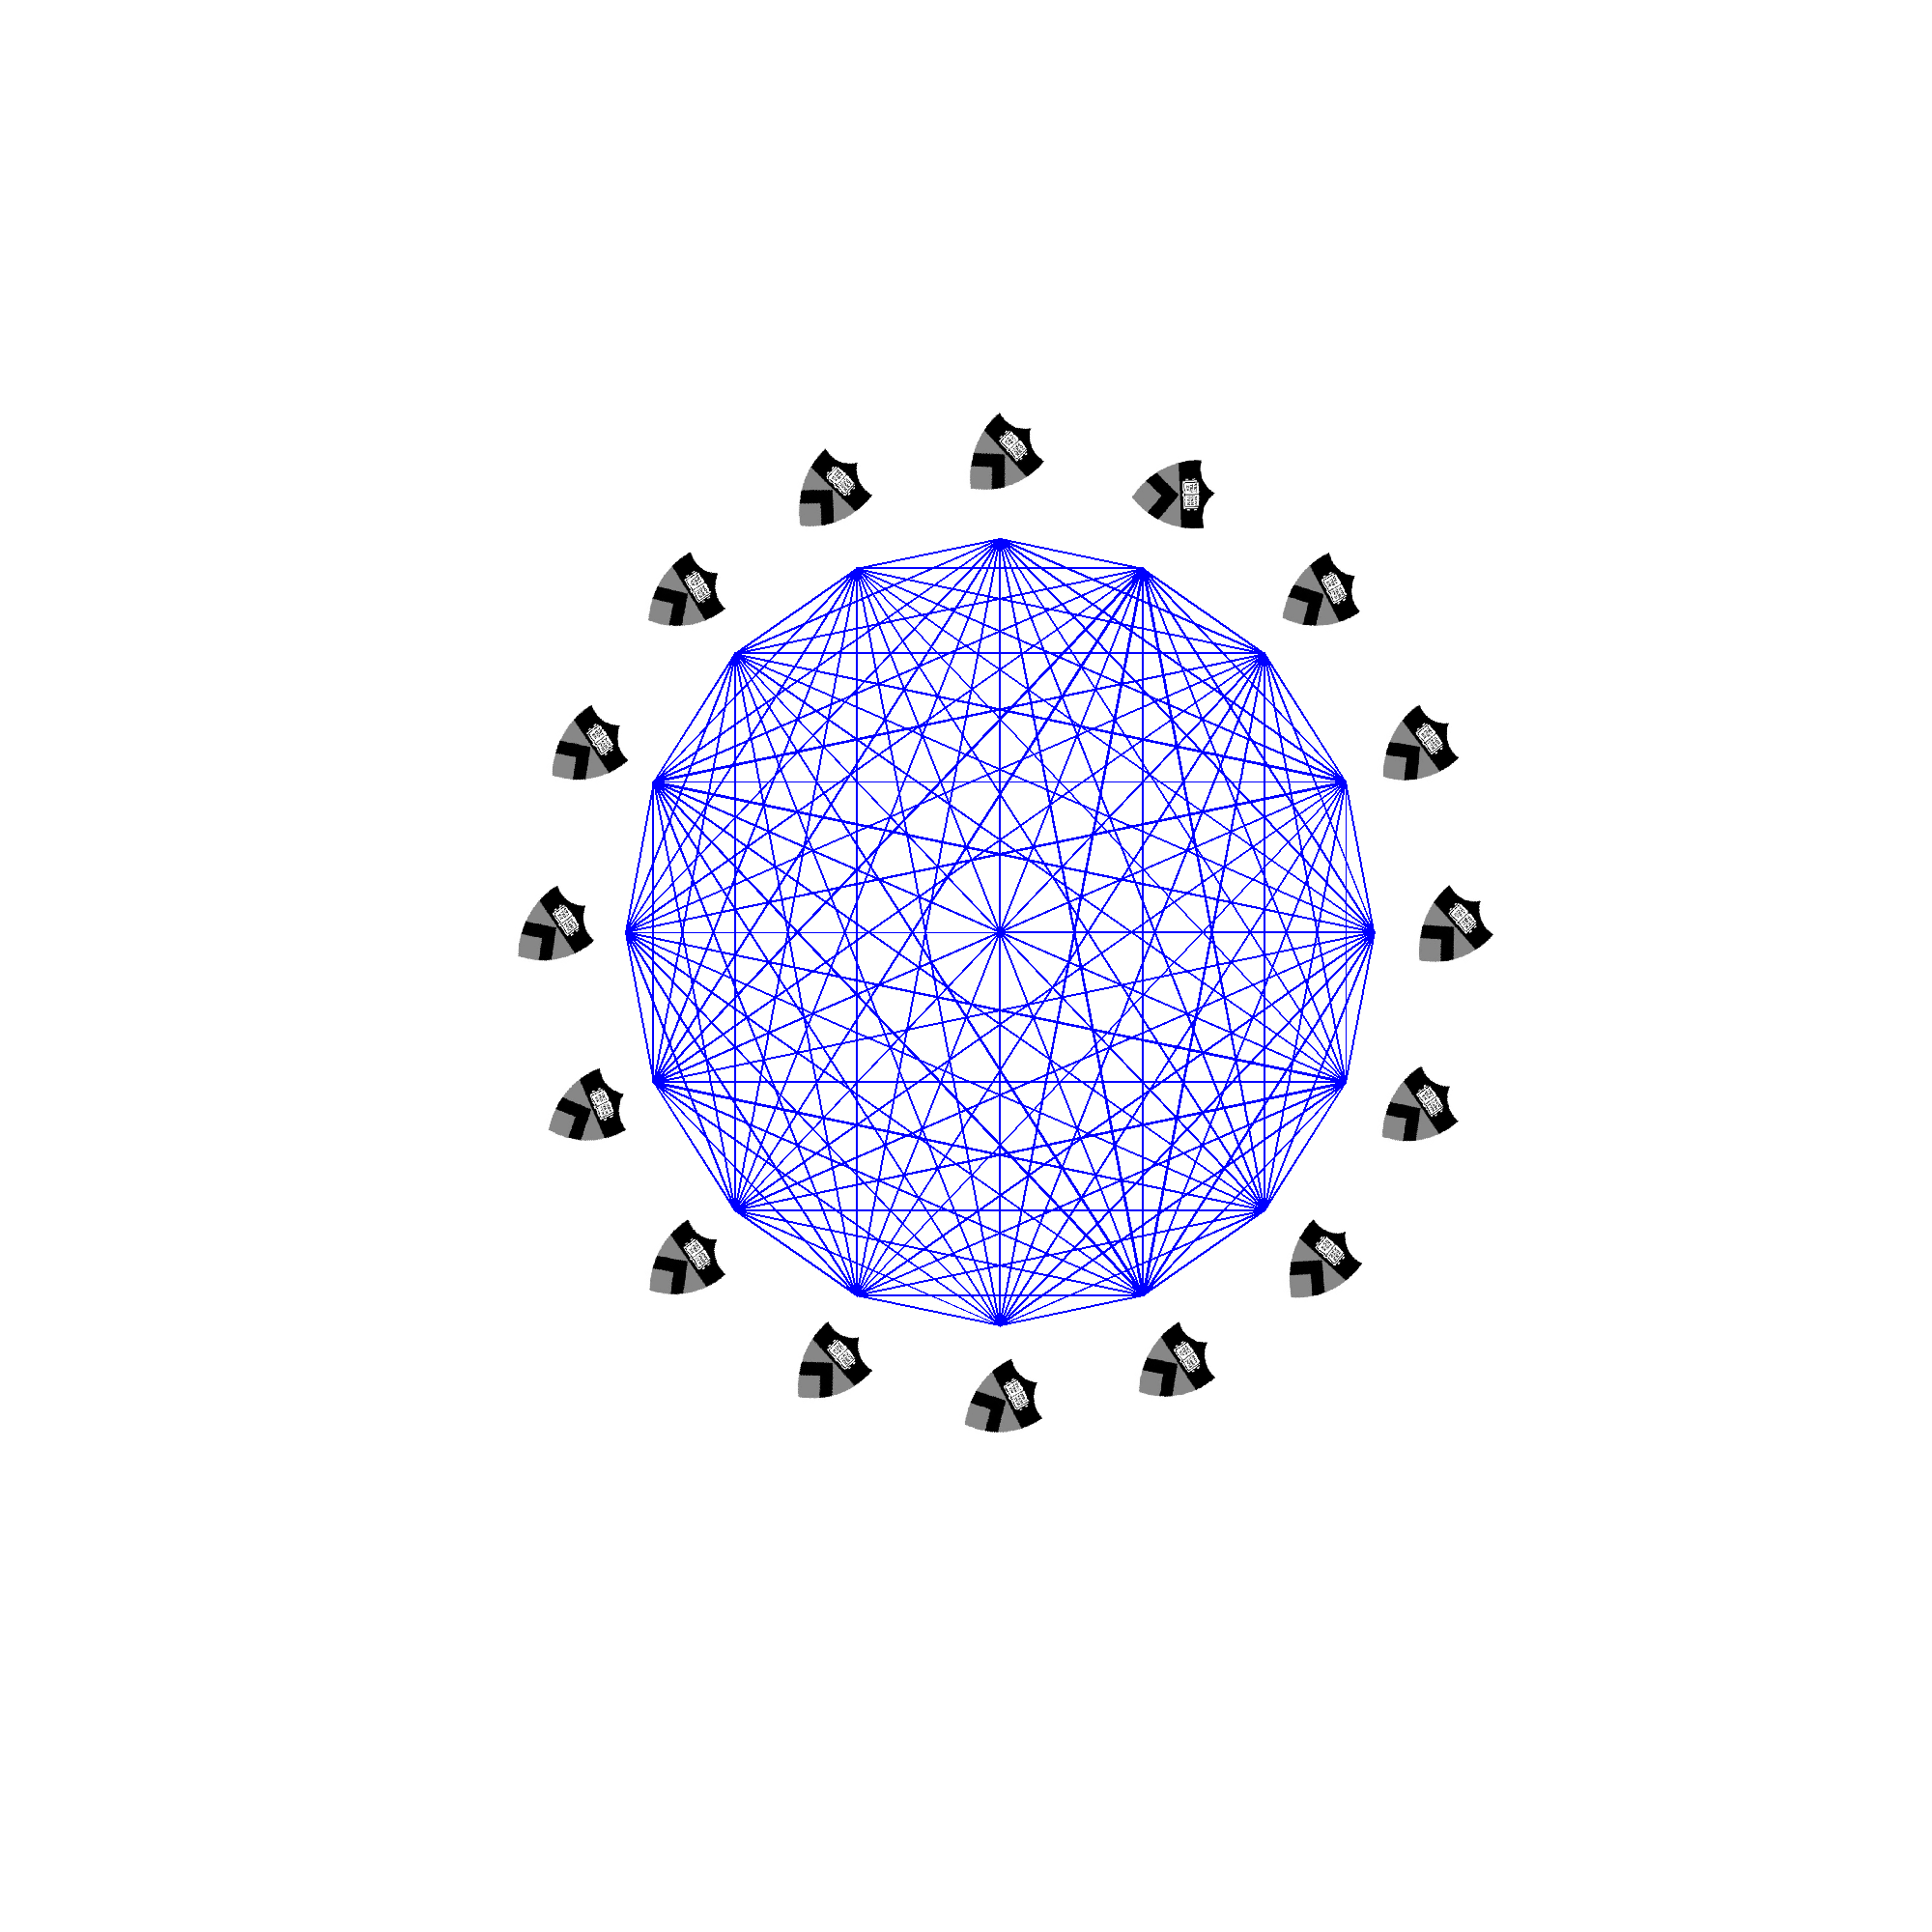
\includegraphics[width=0.9\textwidth]{PU_angsynch3} \\
	{\small \em Images, aligned using angular synchronization and then denoised. \par}}
	\end{minipage}
	%
	\begin{minipage}[t]{0.4\textwidth}
	{\small
	\begin{itemize}
	\item We compute the angle $\theta_{ij}$ that optimally aligns image $i$ to image $j$ for every pair $i, j$.
	\item We want to find angles $\theta_1, \dots, \theta_n$ such that $\theta_i -  \theta_j \approx \theta_{ij}$.
	\item We also want to satisfy {\em higher-order} consistency, e.g. we not only want $\theta_i - \theta_j \approx \theta_{ij}$, but also $\theta_i - \theta_j \approx \theta_{ik} + \theta_{kj}$. 
	\end{itemize}
	\par}
	\end{minipage}
	
\end{frame}

\begin{frame}{Angular Synchronization for Data Alignment}

	\begin{block}{Angular Synchronization Algorithm \footnotemark}
		{\scriptsize 
		 We have {\bf data} $x_1, x_2, \dots, x_n$ (e.g., $x_i$ is the concentration profile of dpERK on a ring).
        
        $\theta_{ij}$ denotes the {\bf angle of rotation} that best aligns $x_i$ and $x_j$.

        We {\bf construct the matrix} $H$, where $H_{ij} = e^{i \theta_{ij}}$.

		The entries of $v_1$, the {\bf top eigenvector} of $H$, contain estimates of the optimal rotations for each data point.

		The optimal rotations $\hat{\theta_1}, \dots, \hat{\theta_n}$ are given by $e^{i \hat{\theta_i}} = \frac{v_1(i)}{|v_1(i)|}$.
		\par}
	\vspace{-0.9in}
	\hspace{0.85\textwidth}
	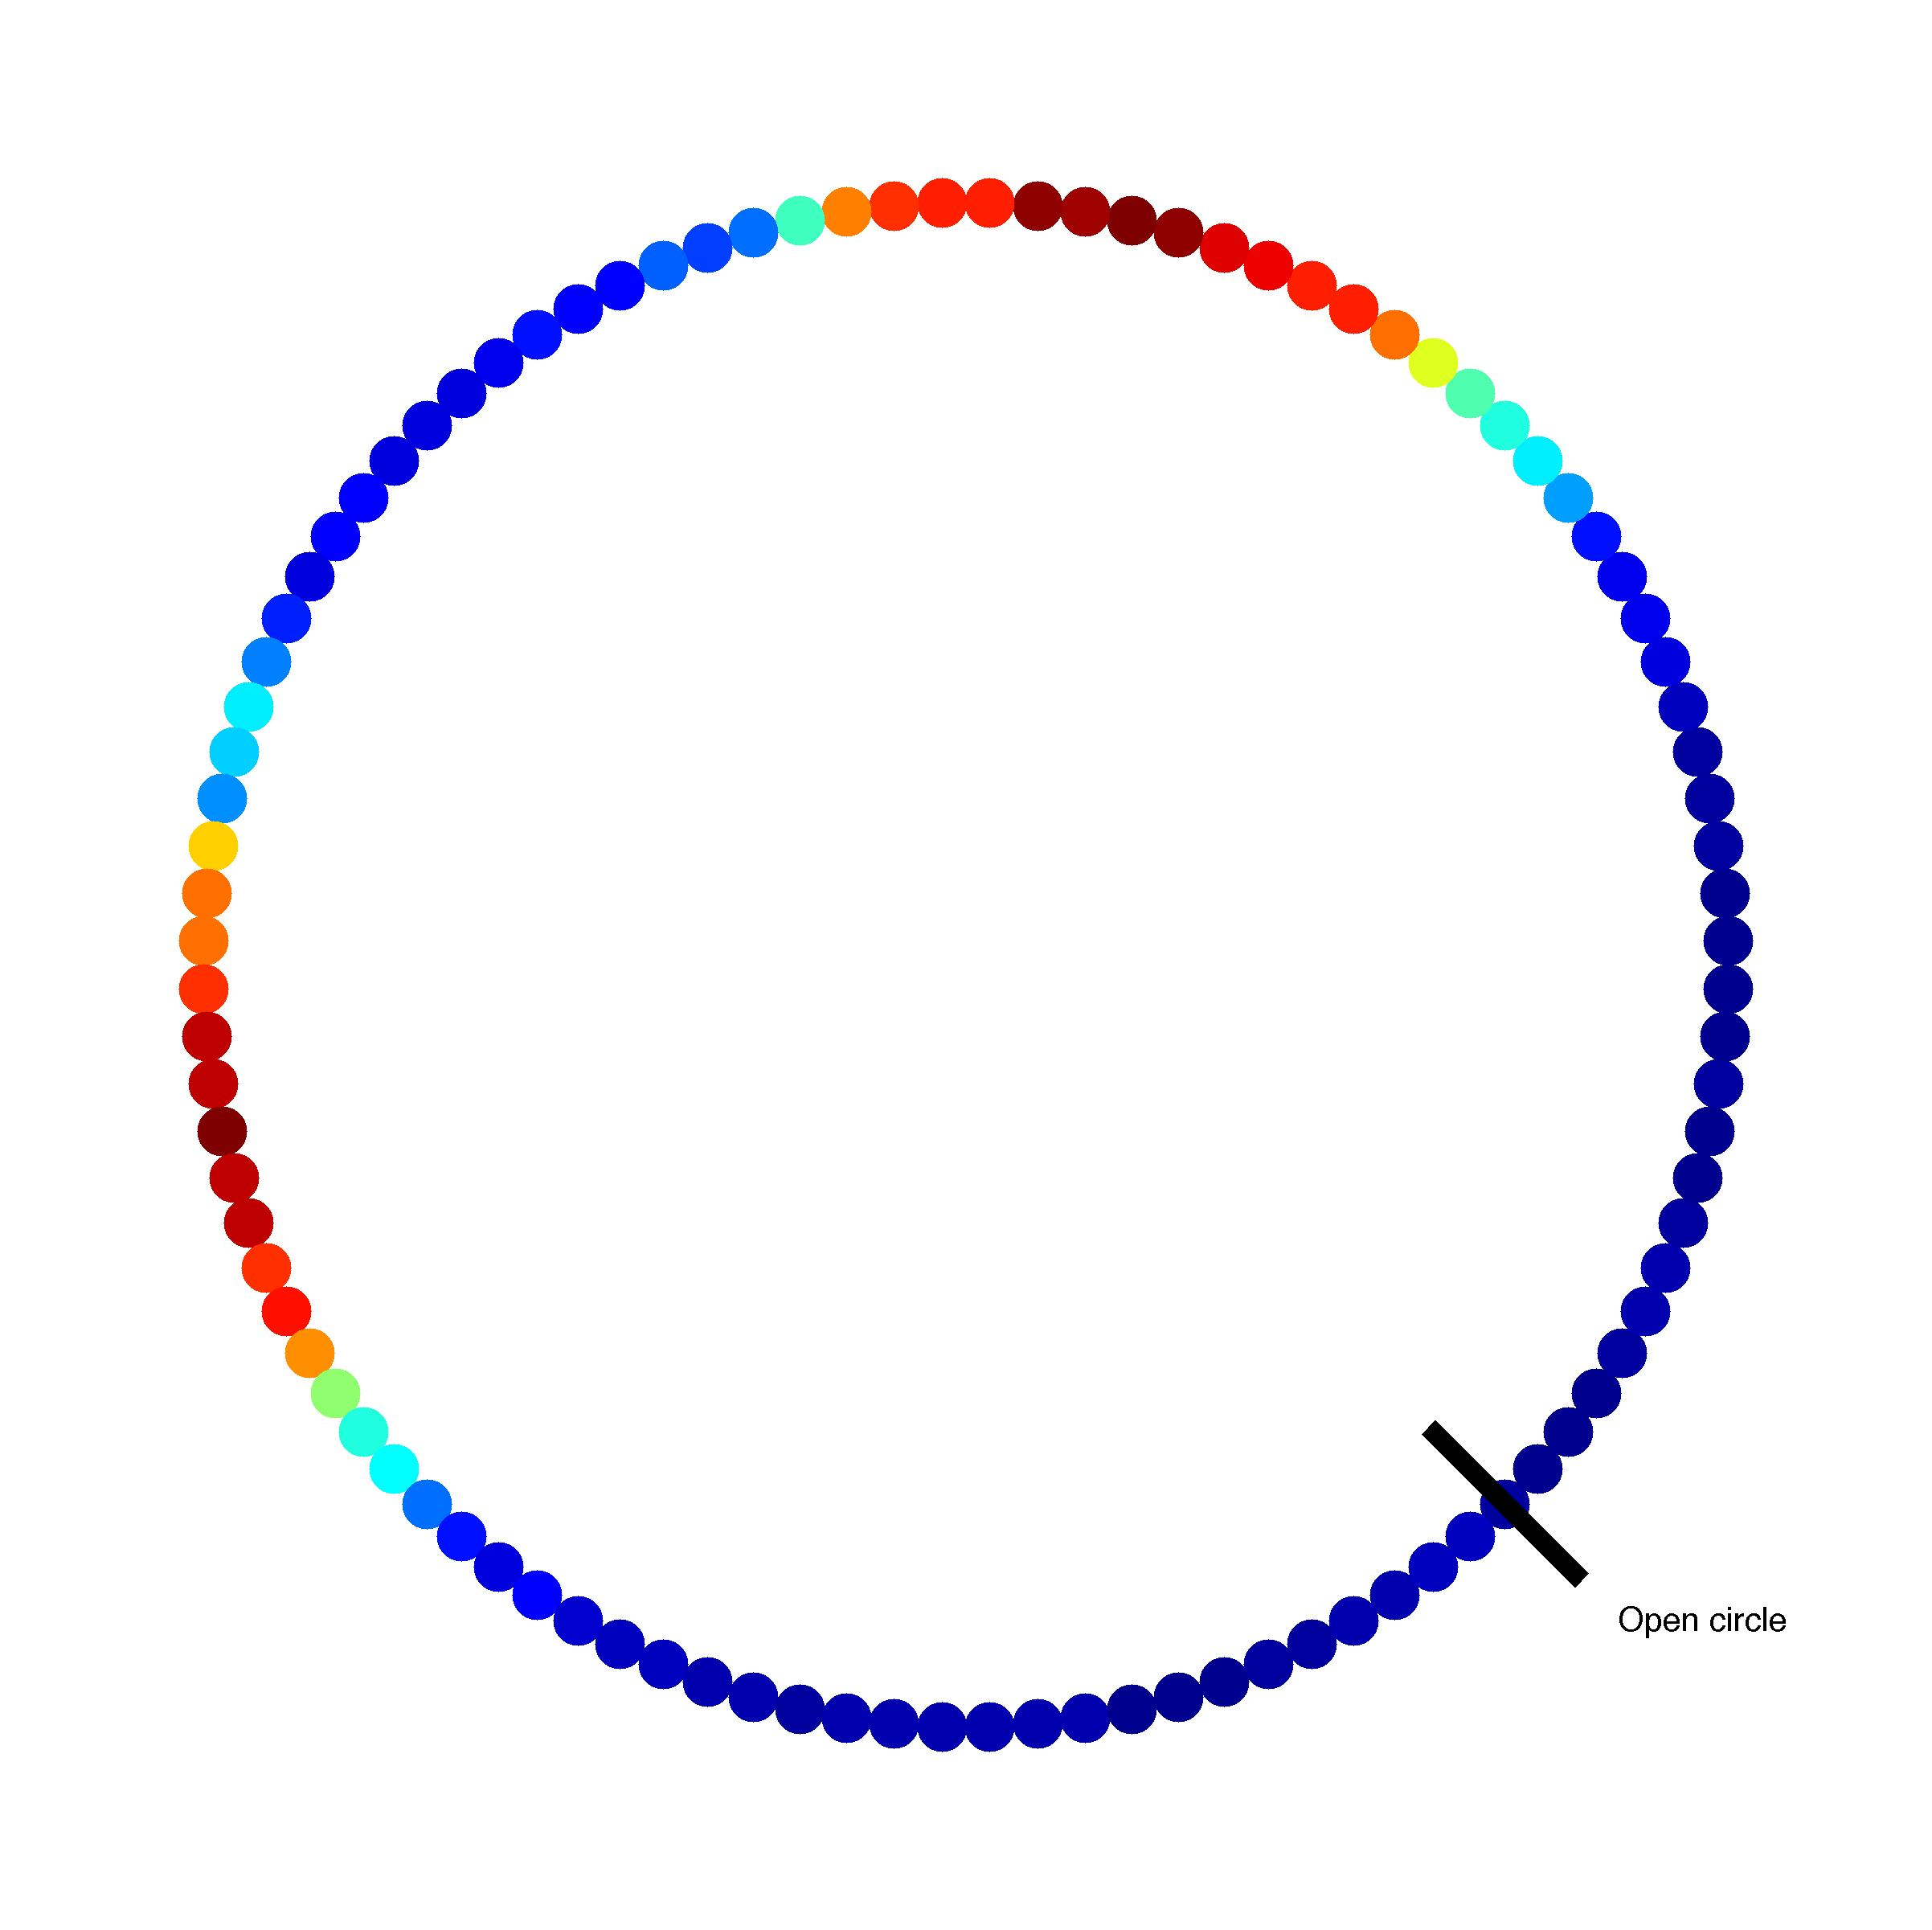
\includegraphics[width=0.1\textwidth]{circle_profile}
	\vspace{0.4in}	
	\end{block}	
	\footcitetext{singer2011angular}
	
	\vspace{-0.1in}
	We can use angular synchronization to align the concentration profiles
	
	\begin{tikzpicture}
		\node[] (fig1) {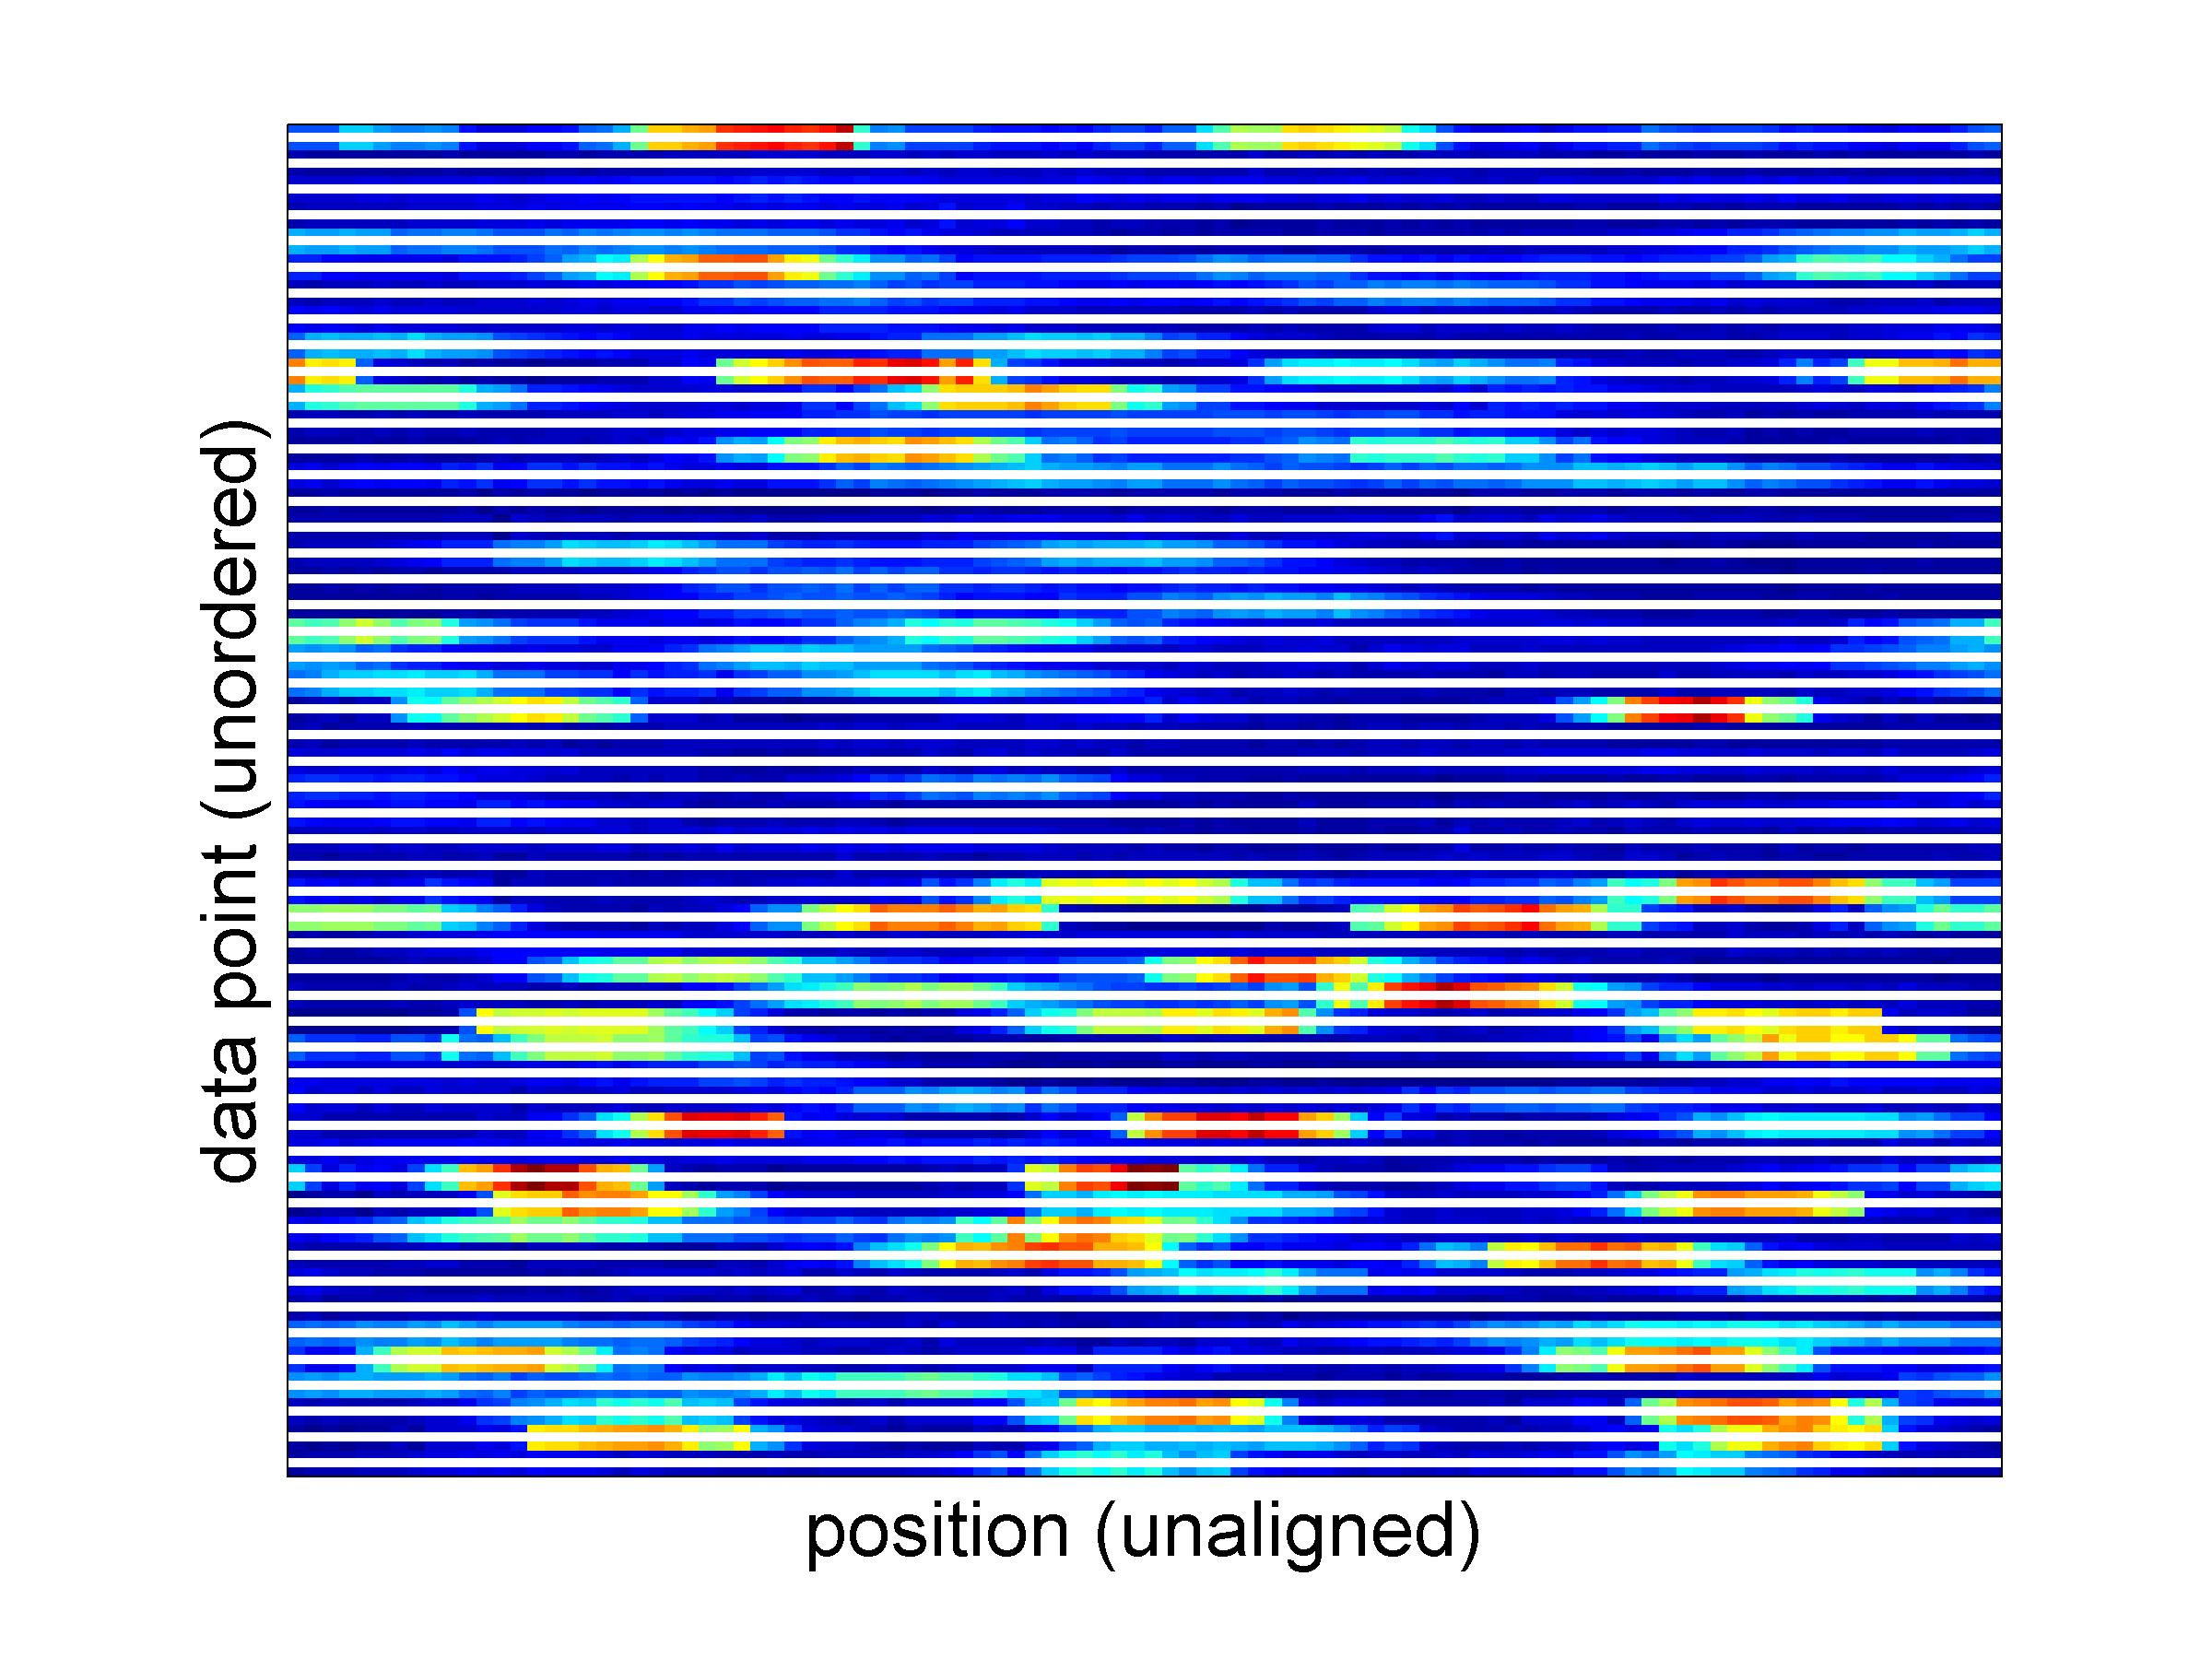
\includegraphics[width=0.25\textwidth]{data_unaligned_unordered_spaced}};
		\node[right of=fig1, node distance=0.35\textwidth] (fig2) {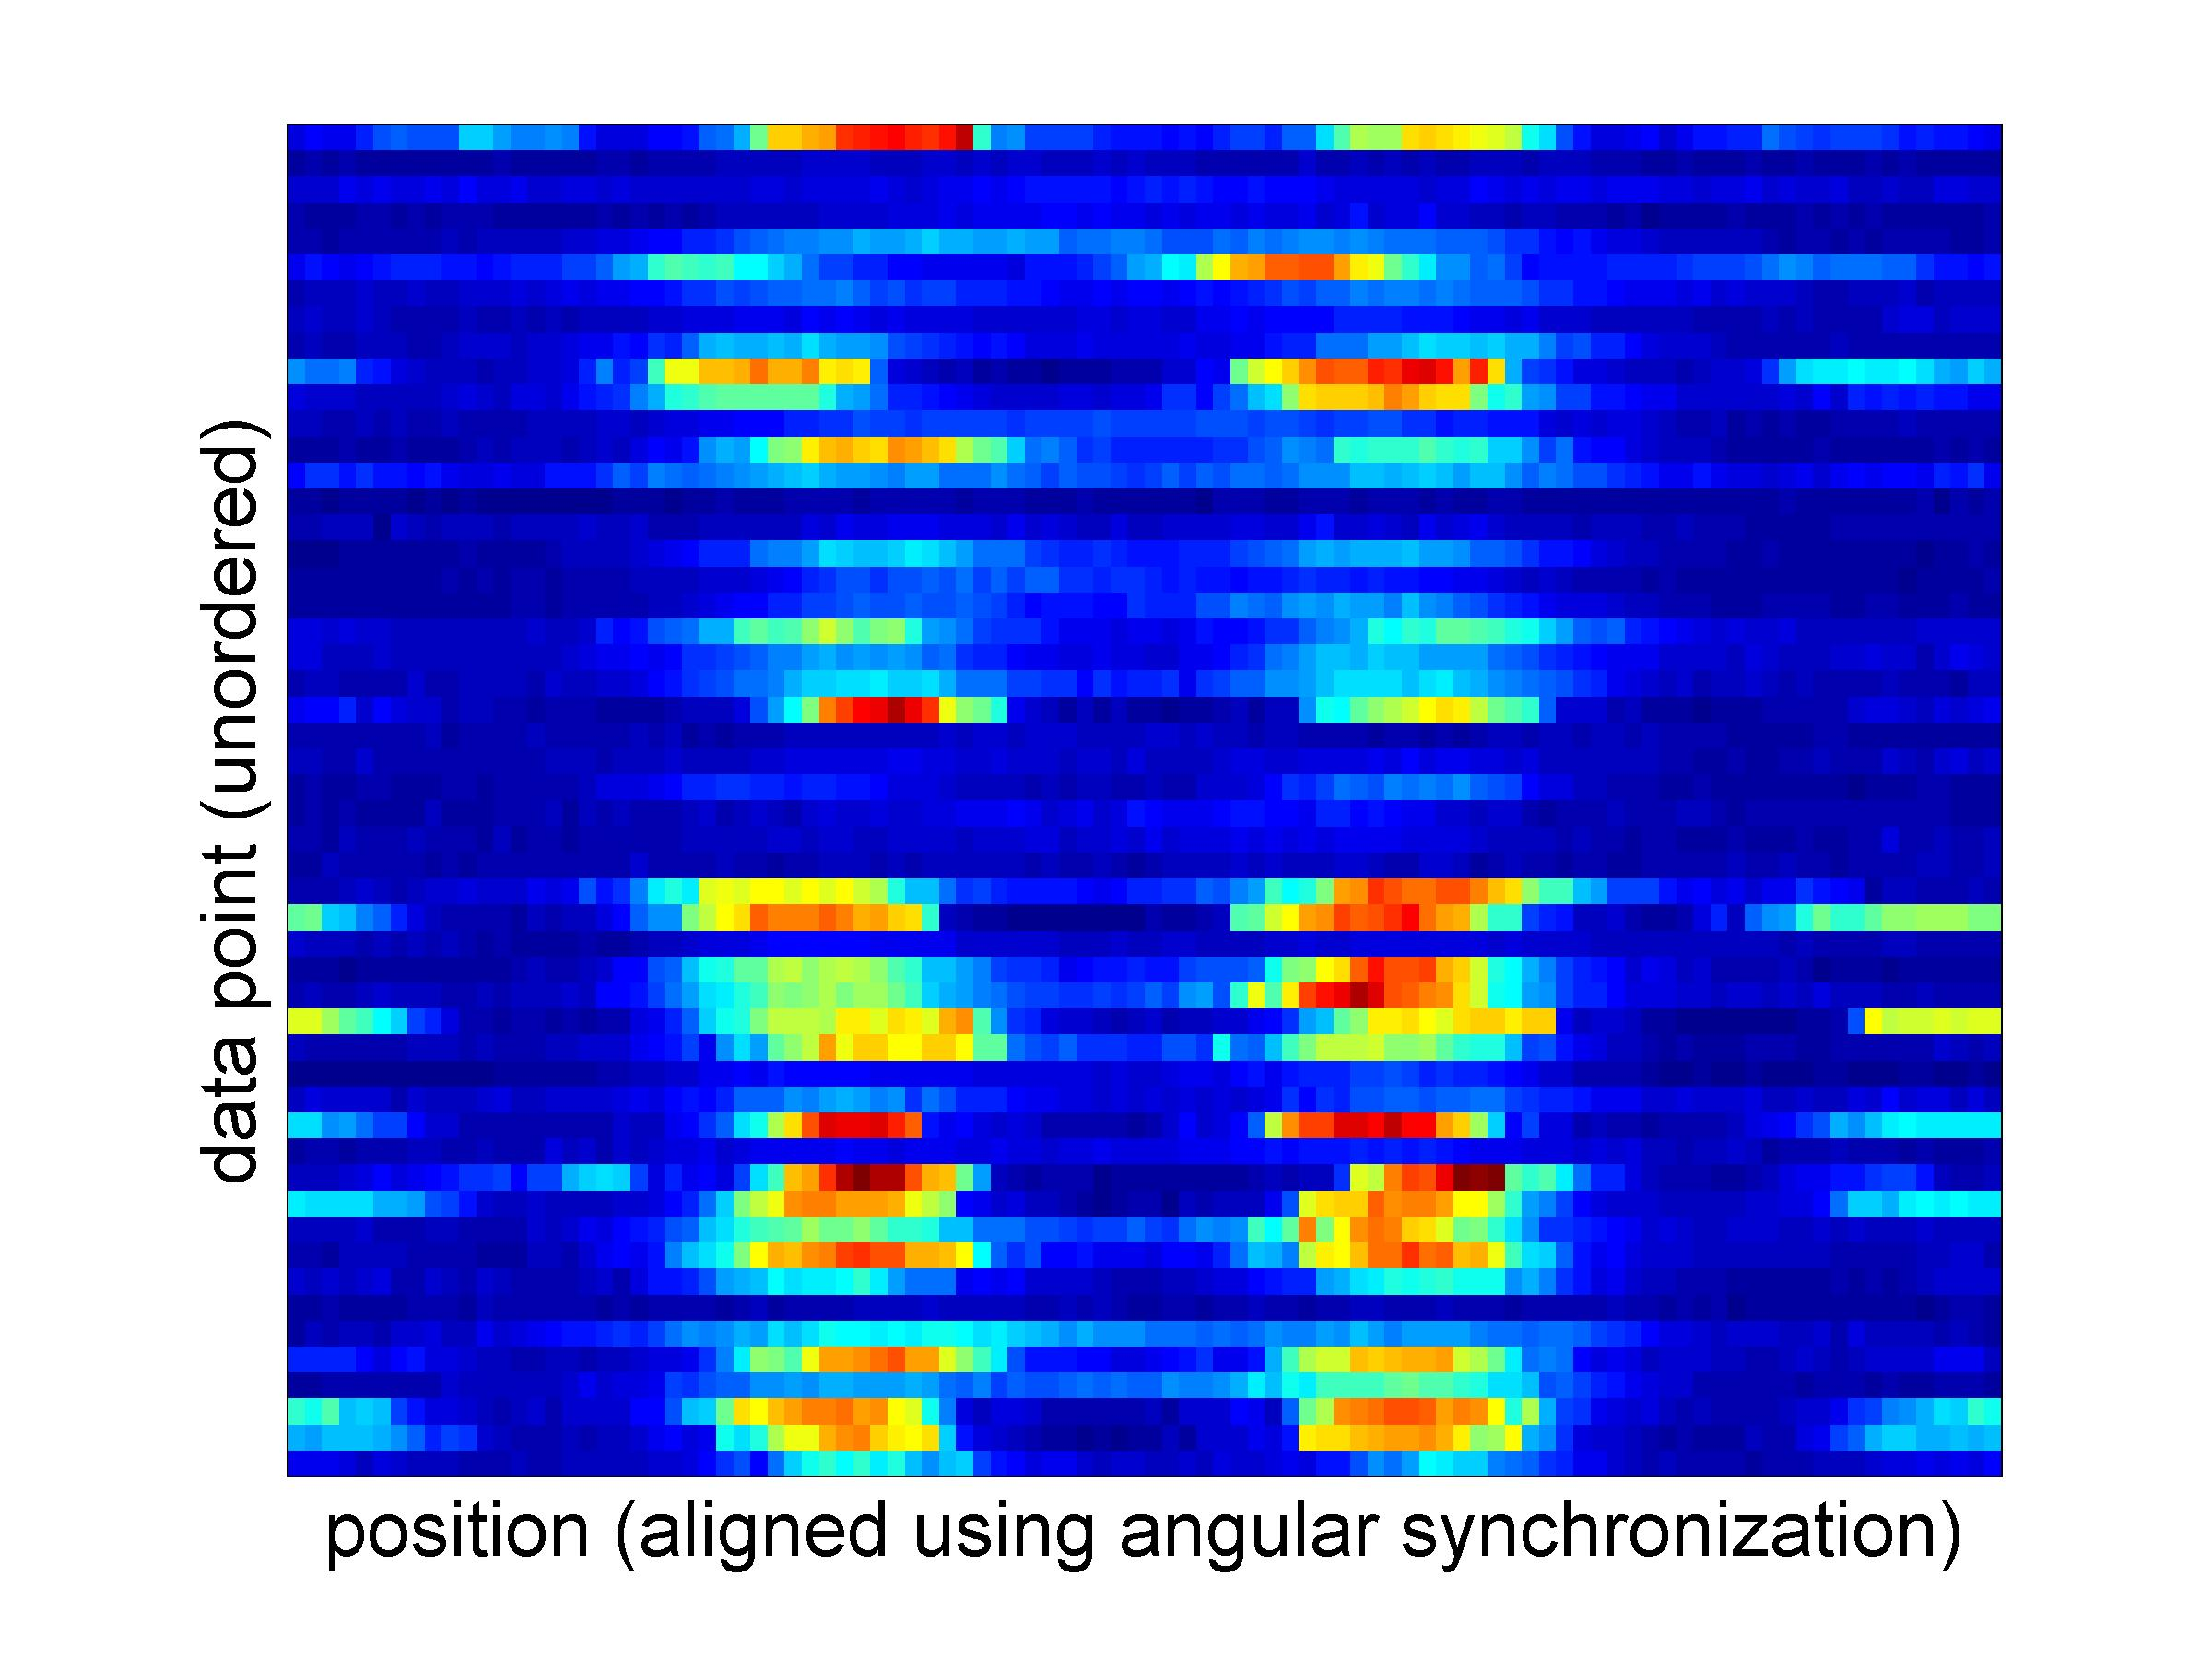
\includegraphics[width=0.25\textwidth]{data_aligned_unordered}};
		\node[right of=fig2, node distance=0.35\textwidth] (fig3) {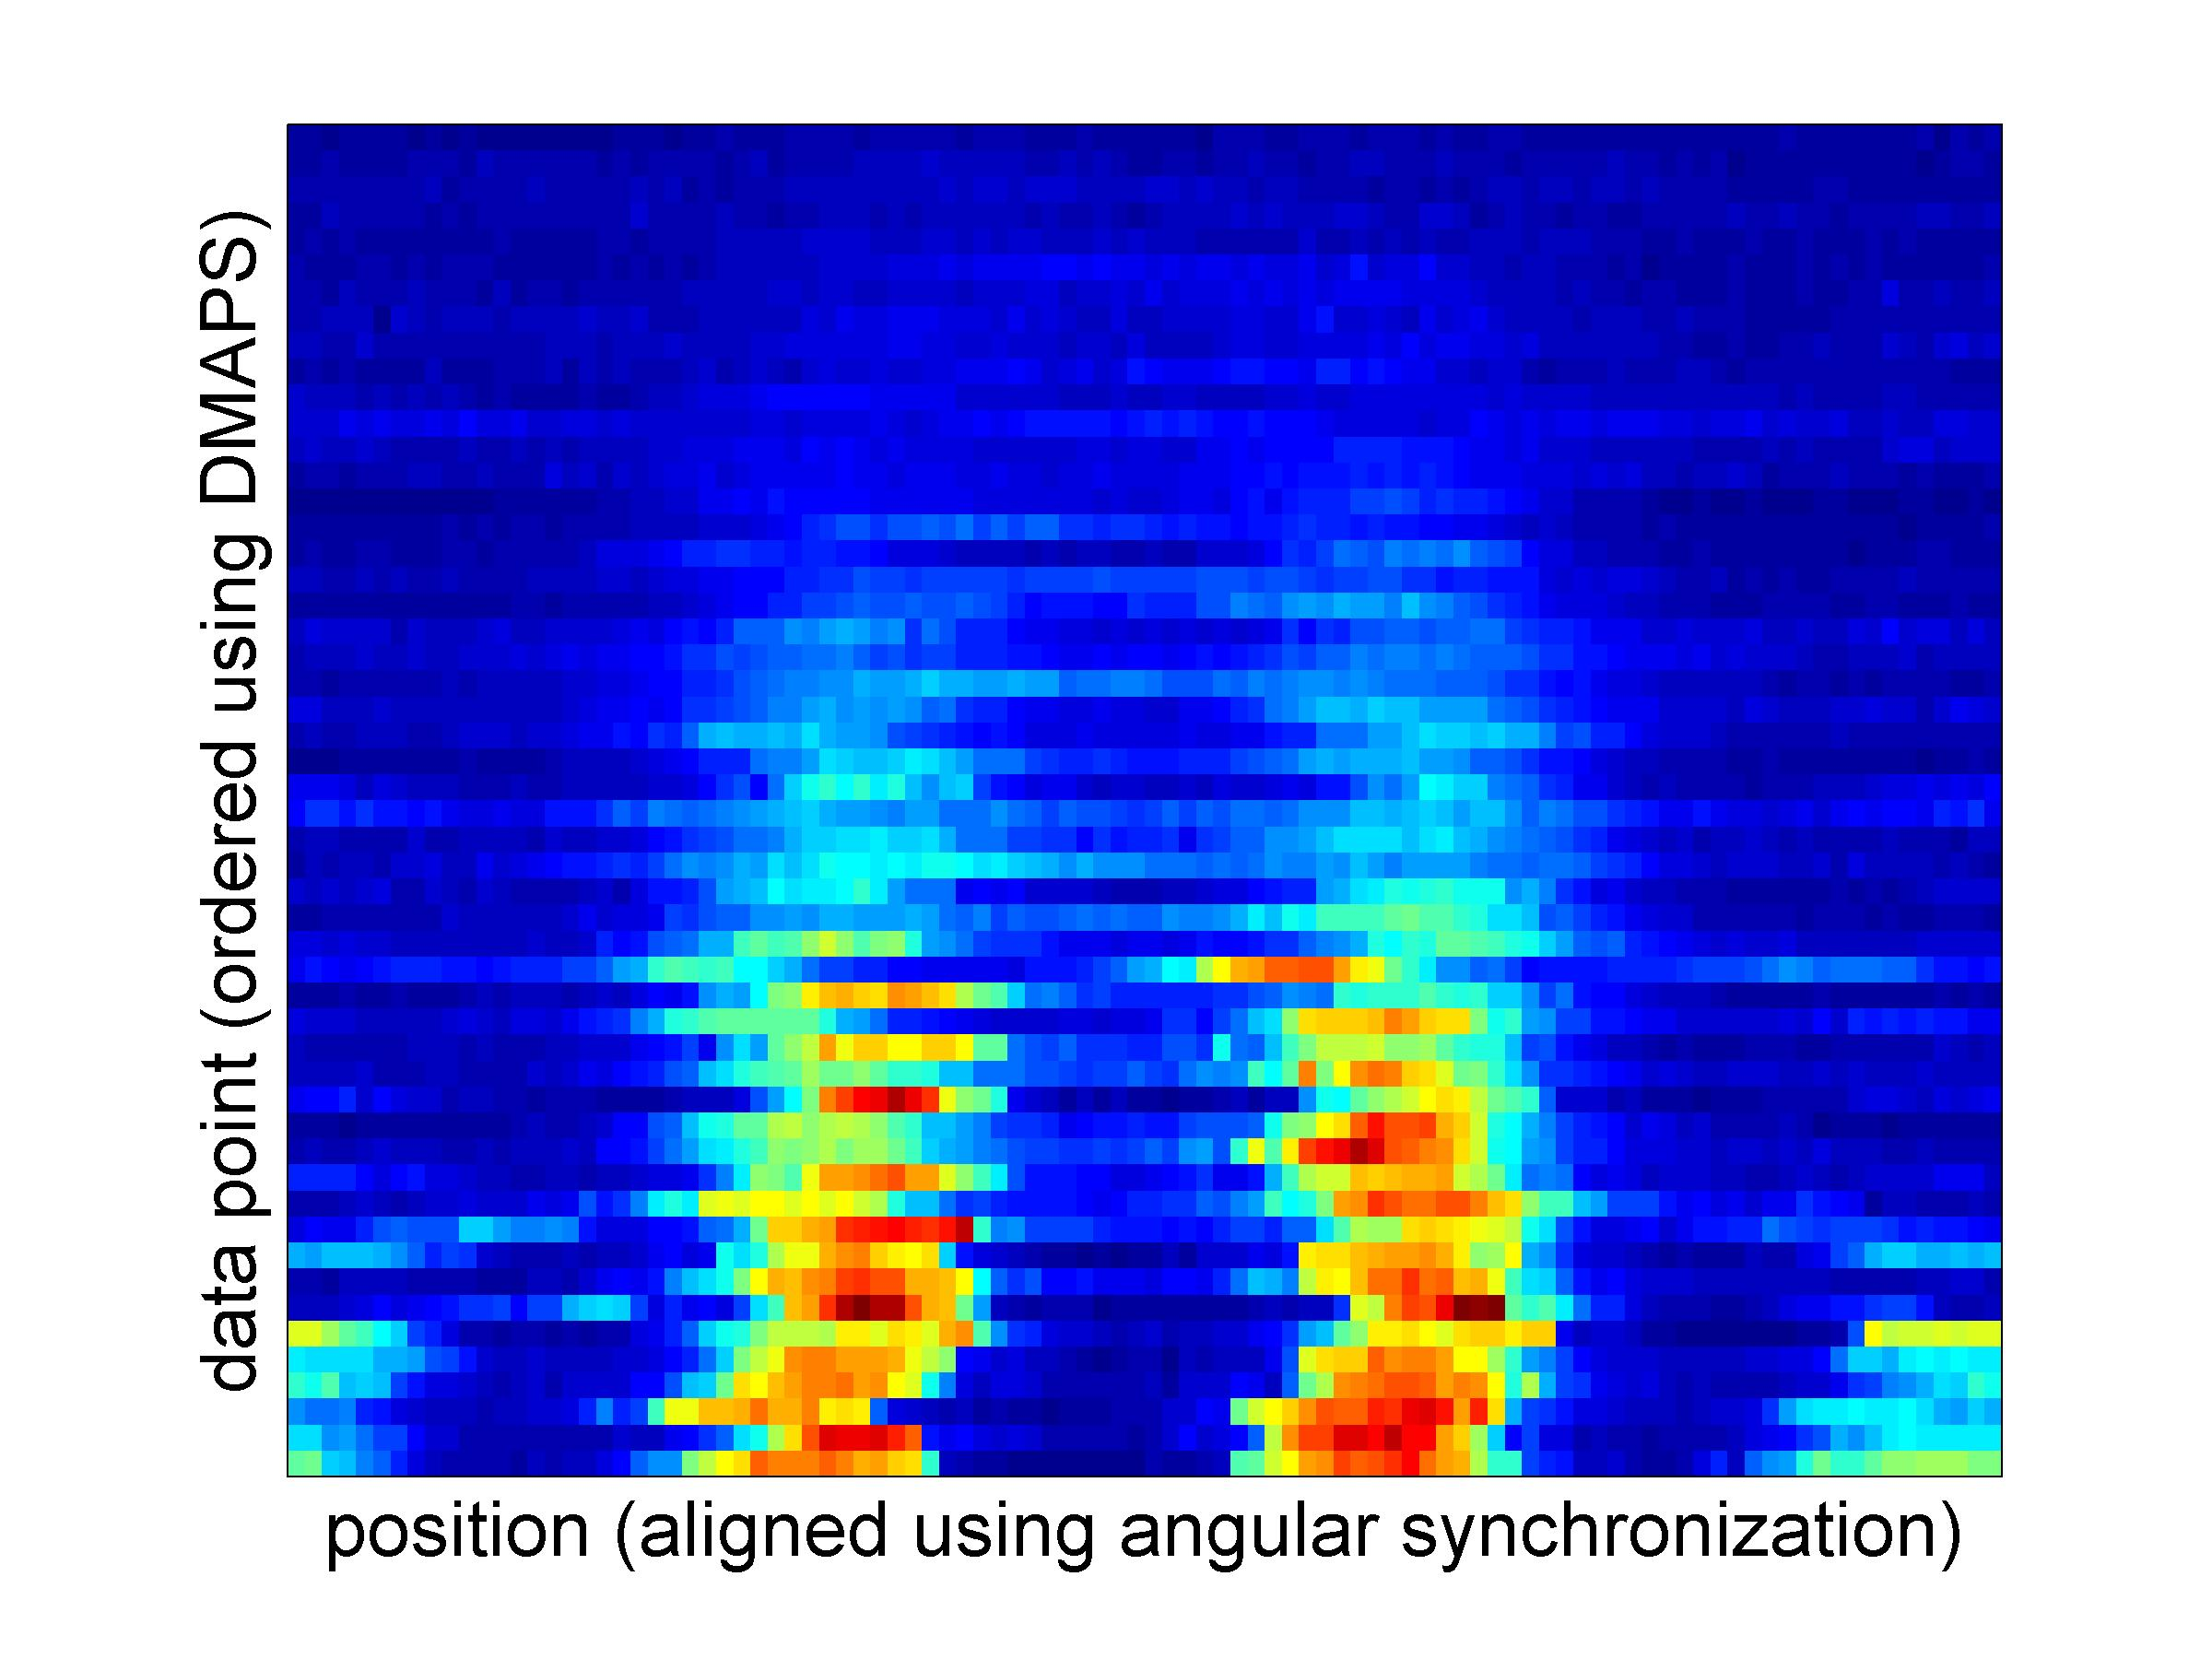
\includegraphics[width=0.25\textwidth]{data_ordered_angsynch}};
		\draw[->] (fig1.east) -- (fig2.west);
		\draw[->] (fig2.east) -- (fig3.west);
		\node[below of=fig1, node distance=0.7in, text width=0.3\textwidth]{{\scriptsize Profiles are unaligned and unordered. We are allowed to shift the profiles left and right (this corresponds to rotations of the circular profiles). \par}};
		\node[below of=fig2, node distance=0.7in, text width=0.3\textwidth]{{\scriptsize Profiles are aligned using angular synchronization but temporally unordered. \par}};
		\node[below of=fig3, node distance=0.7in, text width=0.3\textwidth]{{\scriptsize Profiles are then ordered in time using DMAPS. \par}};
	\end{tikzpicture}

\end{frame}

\begin{frame}{Vector Diffusion Maps: Synchronization and DMAPS}
	%Our data contains both symmetries {\em and} dynamics
	
	\begin{minipage}{0.45\textwidth}
	\begin{block}{Diffusion maps}
		Calculate top eigenvectors of $W$, where $W_{ij} = e^{-\frac{d^2(x_i, x_j)}{\epsilon}} / \sum_j e^{-\frac{d^2(x_i, x_j)}{\epsilon}} $
	\end{block}
	\end{minipage}	
	\hfill
	\begin{minipage}{0.45\textwidth}	
	\begin{block}{Angular Synchronization}
		Calculate top eigenvector of $H$, where $H_{ij} = e^{-i \theta_{ij}}$
	\end{block}
	\end{minipage}
	
	\begin{block}{Vector Diffusion Maps (VDM) \footnotemark} 
		Calculate the top eigenvectors of $S$, where $S_{ij} = W_{ij}H_{ij}$
		
		The top eigenvectors then give us the optimal rotations {\em and} the embedding coordinates for our data
	\end{block}
	\footcitetext{singer2012vector}

	\vspace{-0.2in}
	\begin{tikzpicture}
		\node[] (fig1) {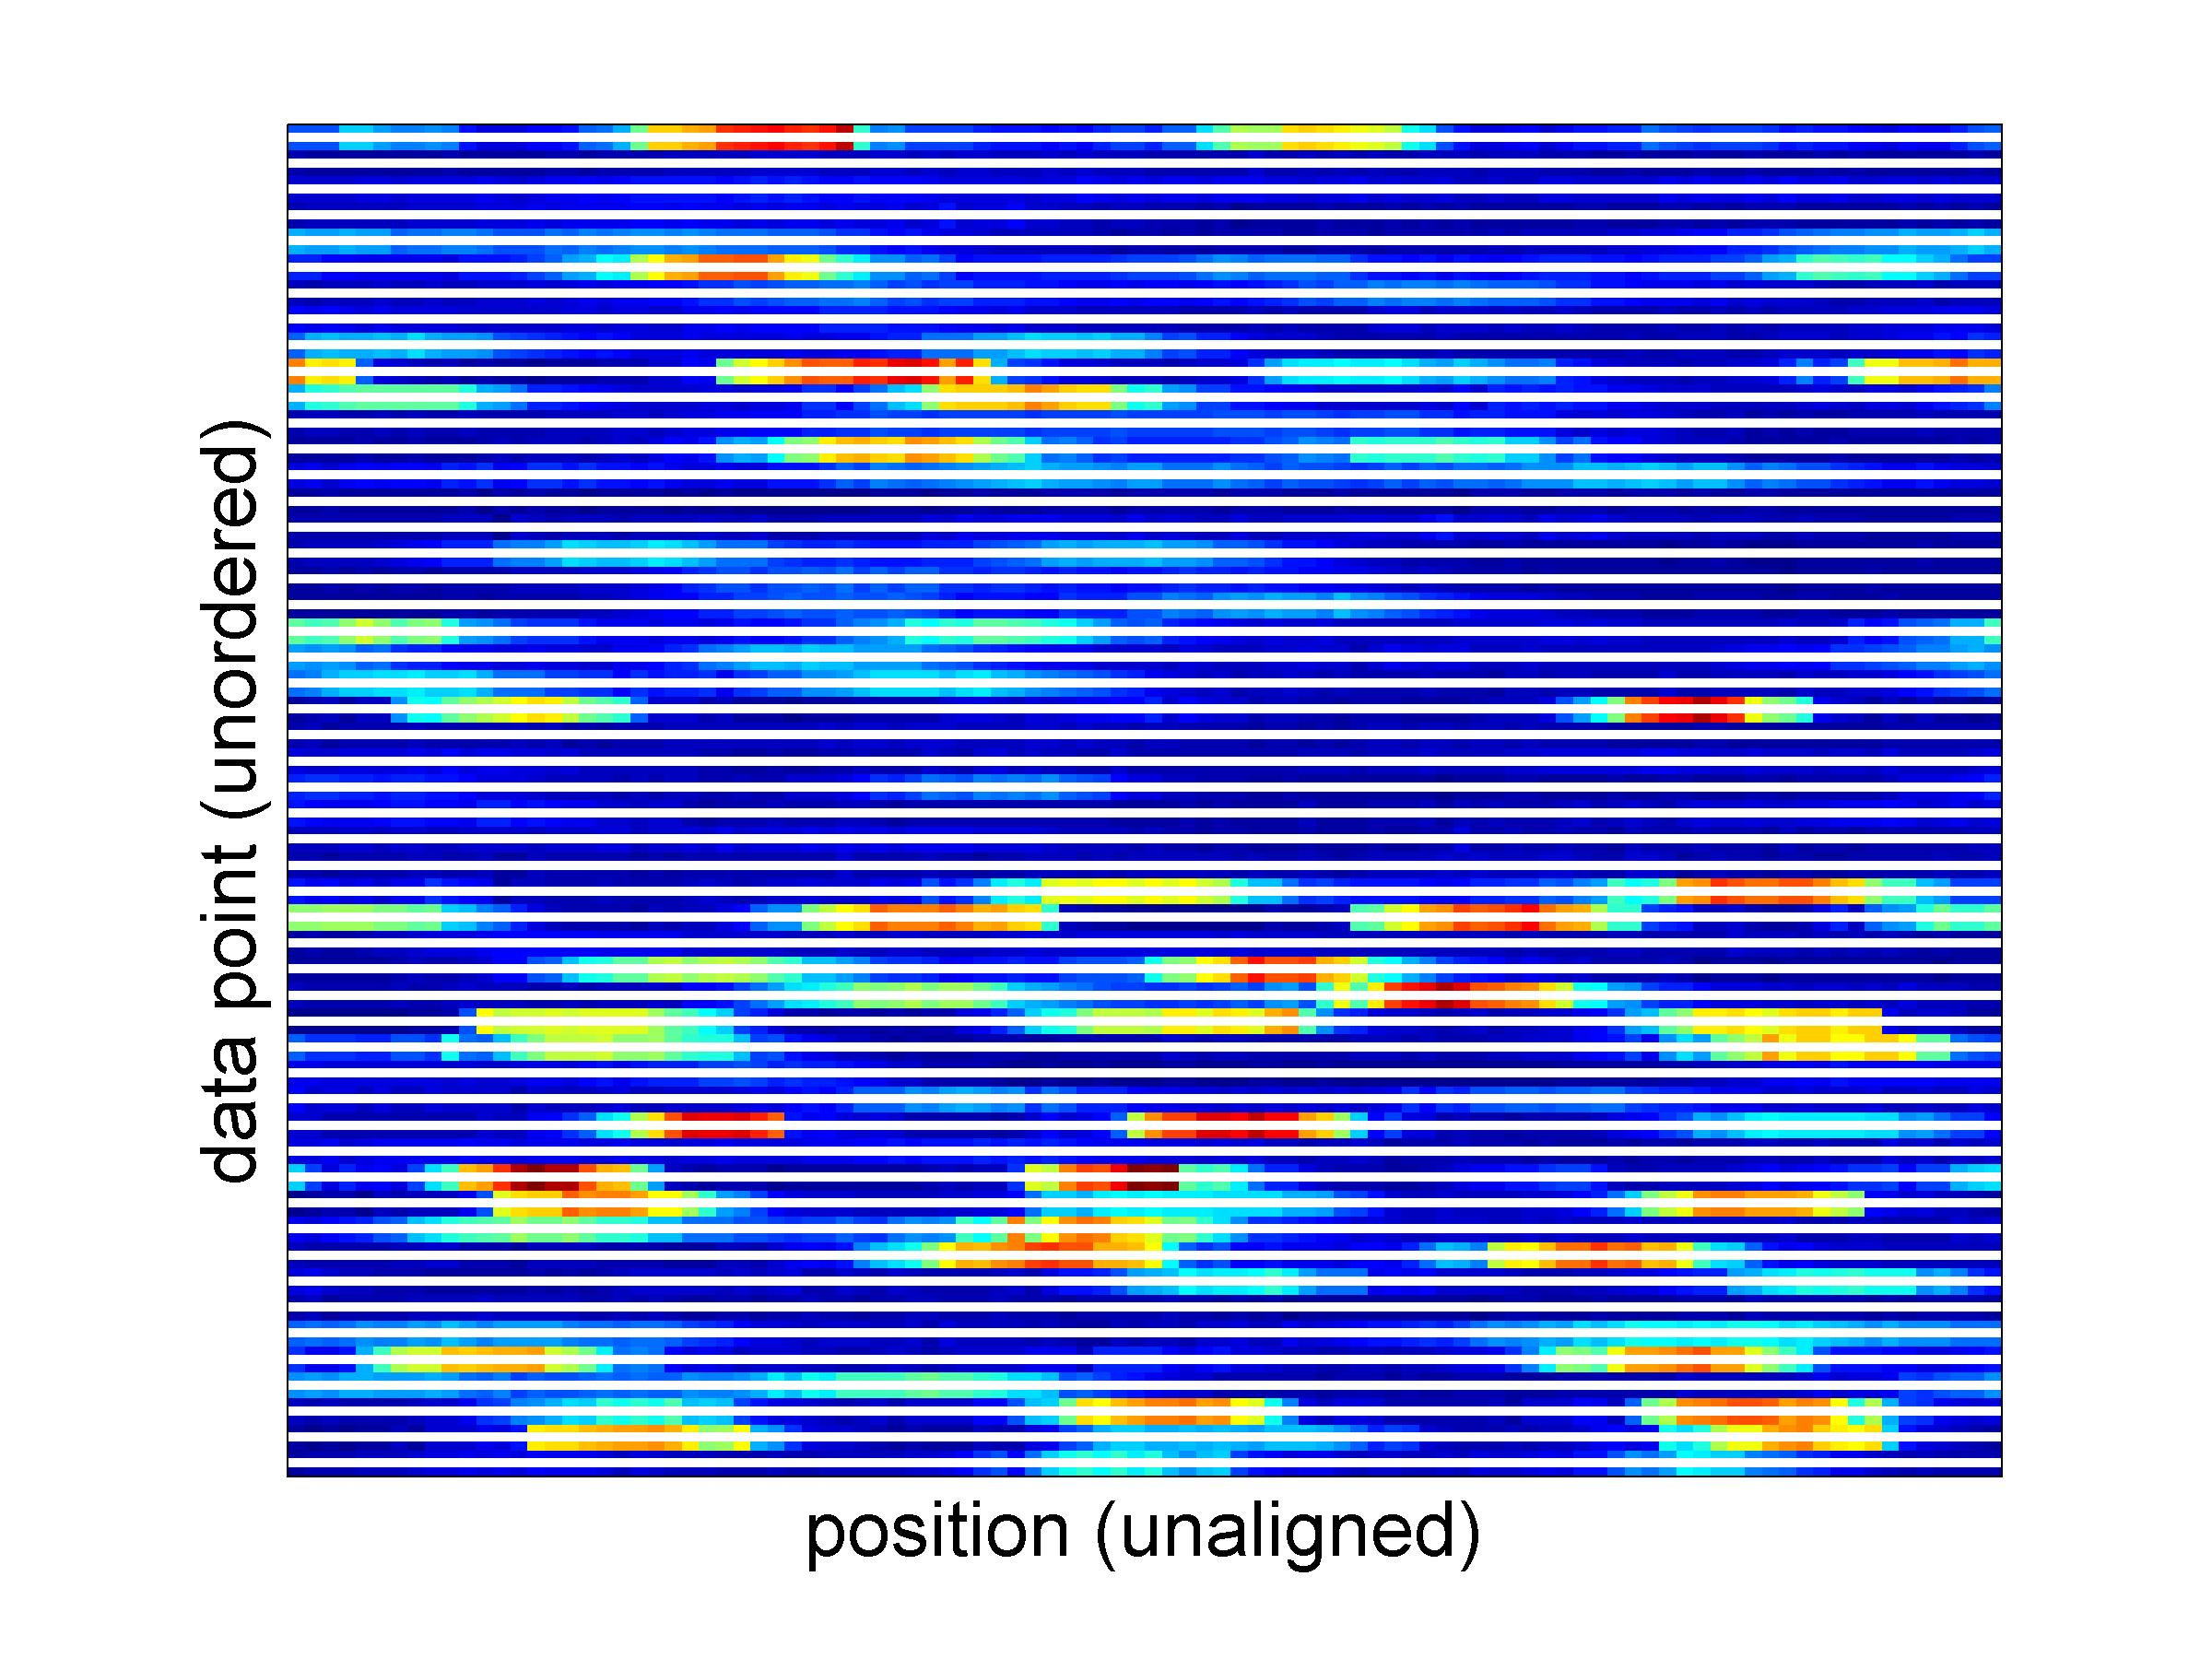
\includegraphics[width=0.3\textwidth]{data_unaligned_unordered_spaced}};
		\node[right of=fig1, node distance=0.6\textwidth] (fig2) {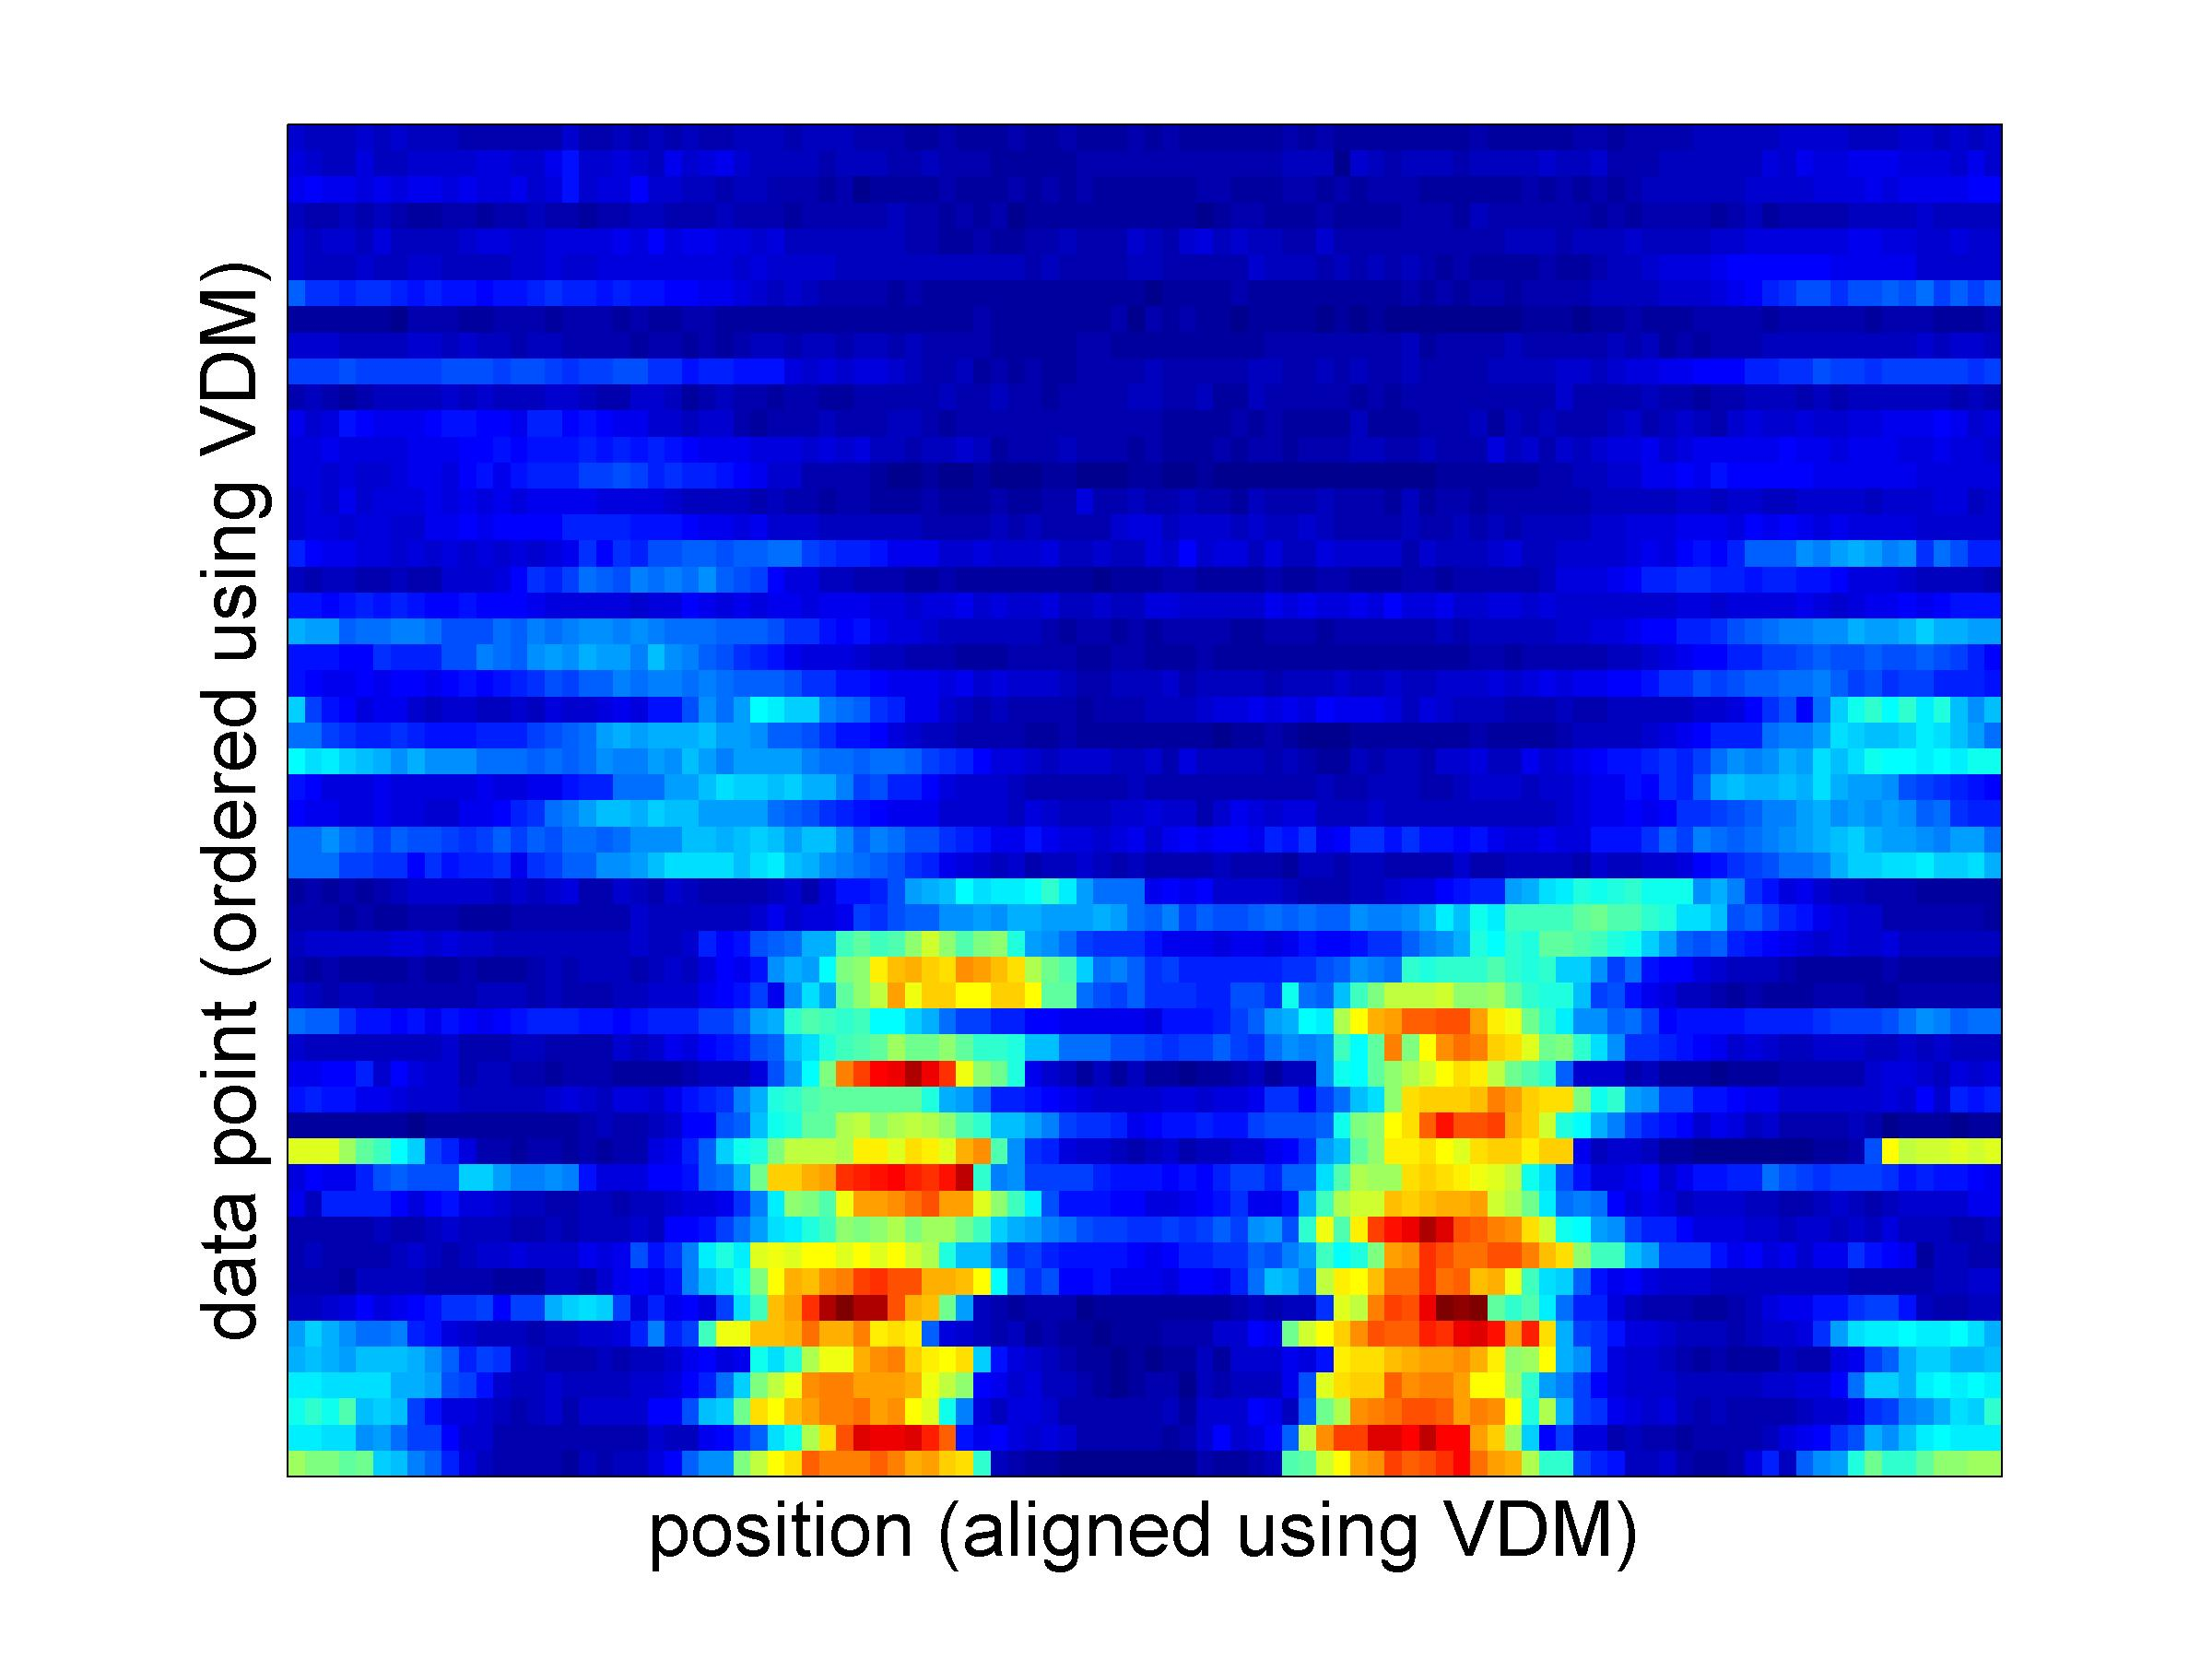
\includegraphics[width=0.3\textwidth]{data_ordered_vdm}};
		\draw[->] (fig1.east) -- (fig2.west) node[above,midway, text width=0.3\textwidth, align=center] { Aligned {\em and} ordered using VDM};
		%\node[below of=fig1, node distance=0.7in, text width=0.4\textwidth]{{\small Profiles are unaligned and unordered \par}};
		%\node[below of=fig2, node distance=0.7in, text width=0.4\textwidth]{{\small Profiles are aligned and ordered using vector diffusion maps} \par };
	\end{tikzpicture}

\end{frame}